% ===========================================================================
%  G4RW Technote -- DUNE ND-LAr 2x2
%  VERSION 2, updated against the September 2026 ND Prototypes Analysis
%  Workshop deck (g4rw_systematics_workshop_September2026_v2.pdf, 32 slides).
%
%  Build:  pdflatex main_v2_sep2026 ; bibtex main_v2_sep2026 ;
%          pdflatex main_v2_sep2026 ; pdflatex main_v2_sep2026
% ===========================================================================
\documentclass[%
article,
nofootinbib
]{revtex4-2}

\usepackage{setspace}
\usepackage{graphicx}
\graphicspath{{figures/}}
\usepackage{bm}
\usepackage{float}
\usepackage{amsmath, amsfonts, amssymb}
\usepackage{xcolor}
\usepackage{listings}
\usepackage{enumitem}
\usepackage{longtable}
\usepackage{url}
% NOTE: lineno is deliberately NOT loaded. Loading it (even without calling
% \linenumbers) patches the output routine and makes any listings environment
% that straddles a page boundary fail with
%   "Incomplete \iffalse; all text was ignored after line NN".
\usepackage{multirow}

\usepackage[colorlinks=true, linkcolor=blue, citecolor=blue, urlcolor=blue, breaklinks=true]{hyperref}

% ---------------------------------------------------------------- listings
\definecolor{codebg}{RGB}{248,248,248}
\definecolor{codeframe}{RGB}{200,200,200}
\definecolor{keyword}{RGB}{0,96,180}
\definecolor{comment}{RGB}{80,150,80}
\definecolor{string}{RGB}{180,40,40}
\definecolor{builtin}{RGB}{150,0,150}

\lstnewenvironment{bashcode}
    {\lstset{language=bash}}
    {}

\lstset{
    basicstyle=\ttfamily\small,
    backgroundcolor=\color{codebg},
    frame=single,        % NOT shadowbox: a shadowbox listing cannot break
                         % across a page boundary.
    framerule=0.5pt,
    rulecolor=\color{codeframe},
    breaklines=true,
    showstringspaces=false,
    tabsize=4,
    xleftmargin=8pt,
    xrightmargin=4pt,
    aboveskip=6pt,
    belowskip=4pt,
    captionpos=b,
    language=bash,
    keywordstyle=\color{keyword}\bfseries,
    commentstyle=\color{comment}\itshape,
    stringstyle=\color{string},
    morekeywords={sbatch, srun, shifter, source, export, setup, mkdir, module, cvmfs},
    emph={root, python, g++},
    emphstyle=\color{builtin}\bfseries,
    numbers=left,
    numberstyle=\tiny\color{codeframe},
    numbersep=8pt,
}

\lstnewenvironment{cppcode}
    {\lstset{language=C++}}
    {}

% ---------------------------------------------------------------- shorthand
% Must be robust: these appear inside captions, which revtex writes to the
% .aux/.lot.
\DeclareRobustCommand{\pip}{$\pi^{+}$}
\DeclareRobustCommand{\pim}{$\pi^{-}$}
\DeclareRobustCommand{\pipm}{$\pi^{\pm}$}
\DeclareRobustCommand{\Kpm}{$K^{\pm}$}
\DeclareRobustCommand{\gfour}{\texttt{Geant4}}
\DeclareRobustCommand{\gfrw}{\texttt{G4RW}}

\begin{document}


\title{Hadronic Secondary-Interaction Systematics for the DUNE ND-LAr Demonstrator ($2\times2$) with \texttt{Geant4Reweight}}

\author{Muhammad Bilal Azam ({mazam3@hawk.illinoistech.edu}), Zelimir Djurcic ({zdjurcic@anl.gov})}

\date{\today}

\begin{abstract}
This note documents the implementation of hadronic secondary-interaction (SI) systematic uncertainties for the DUNE ND-LAr Demonstrator (2x2) using Geant4Reweight (G4RW). To enable this, the EDepSim persistency manager was patched to retain full Geant4 trajectories,  exclusive-channel fraction files were produced for charged pions (both $\pi^+$ and $\pi^-$), protons, and neutrons, and the G4RW framework was extended to support nucleon reweighting. Per-track SI weights were then generated for pions, protons, and neutrons and matched to CAF observables using truth-level identifiers. The resulting weights were validated at the single-track and distribution levels and propagated to both reconstructed and truth-level observables, including proton track-length and charged-track multiplicity distributions, alongside GENIE and detector systematic uncertainties. This establishes a reproducible SI systematic framework for 2x2 analyses and provides an important ingredient for upcoming physics measurements. This approach will also work for DUNE ND-LAr. 

%Hadrons produced in neutrino interactions re-interact as they propagate through the liquid argon in the DUNE ND-LAr Demonstrator ($2\times2$), and the cross-sections governing these secondary interactions (SI) carry uncertainties. This note documents the use of Geant4Reweight (G4RW) to evaluate these systematics. To achieve this, the EDepSim persistency manager is patched to retain full trajectories, exclusive channel fraction files are generated for $\pi^+$, $\pi^-$, protons, and neutrons, and the reweighter classes are extended to nucleons. Weights are produced for $\pi^+$, $\pi^-$, protons, and neutrons and propagated to the reconstructed observables alongside GENIE and detector uncertainties.
\end{abstract}

\vspace{40pt}
\maketitle

% \tableofcontents
% \newpage

% ===========================================================================
\section{\label{sec:intro}Introduction}
% ===========================================================================

Neutrino interactions in the DUNE ND-LAr $2\times2$ prototype produce hadrons ---
predominantly protons and charged pions --- which must traverse the liquid argon
before they are reconstructed. Along the way they can scatter elastically, be
absorbed, charge-exchange, or produce additional hadrons. These processes are
collectively referred to as secondary interactions (SI), to distinguish them
from final-state interactions occurring inside the struck nucleus. Secondary interactions change the number, type, and kinematics of the
particles that reach the reconstruction, so the cross sections that govern
them enter every hadronic observable the $2\times2$ measures.
Figure~\ref{fig:event_display} gives a representative example: a simulated
neutrino interaction producing a muon, a proton, and a pion from a common
vertex, reconstructed with SPINE~\cite{spine} and shown alongside the truth
view. The two hadrons in this event are exactly the objects whose
re-interaction probability G4RW is being used to vary.

% SOURCE: slide 2, "Reconstructed Neutrino Interaction in the 2x2 Prototype"
\begin{figure}[H]
    \centering
    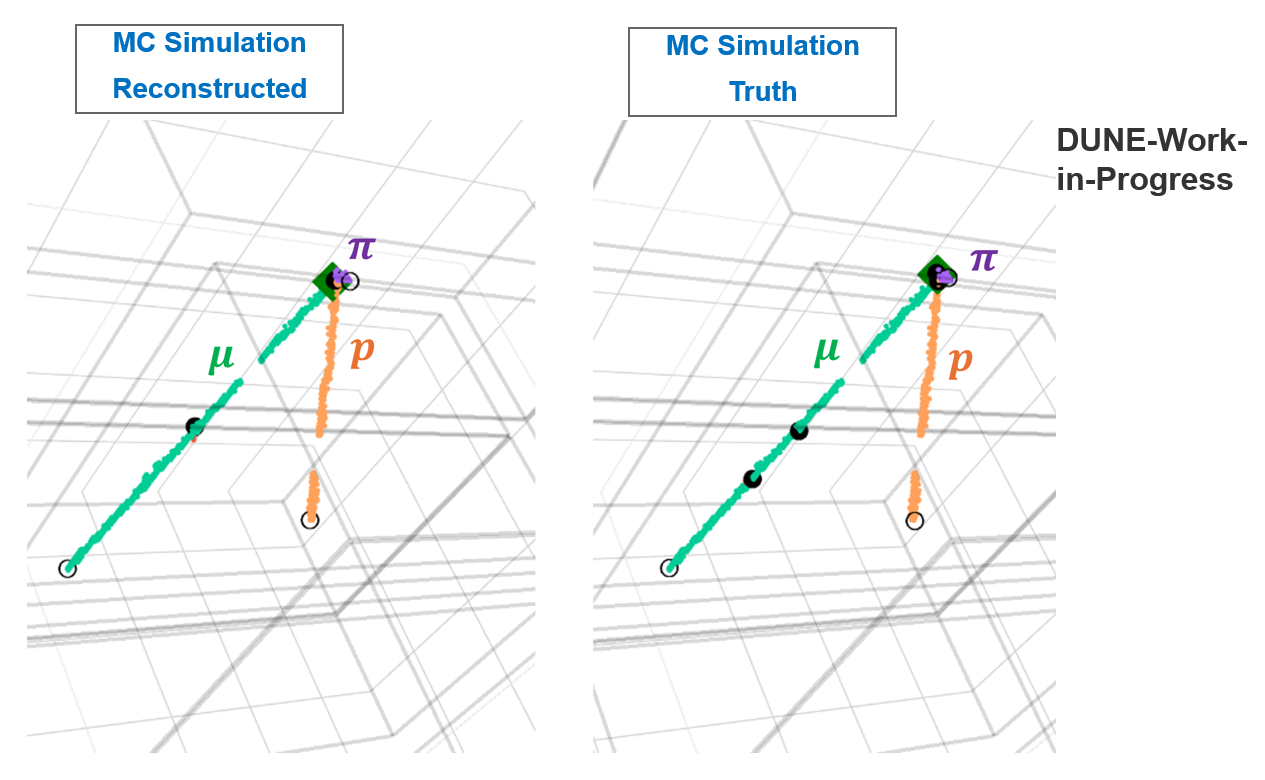
\includegraphics[width=0.82\textwidth]{fig01_event_display}
    \caption{Simulated neutrino interaction in the $2\times2$, shown in the
    reconstructed (left) and truth (right) views. A muon, a proton, and a
    charged pion emerge from a common vertex.}
    \label{fig:event_display}
\end{figure}

Geant4 determines the re-interaction probability using cross sections
looked up from its own internal tables, deciding at each step whether the
particle survives or interacts. Geant4Reweight (G4RW)~\cite{g4rw_paper}
assesses the associated uncertainty by varying those same cross sections
and propagating the resulting shift to physics observables.

That SI uncertainty is one of several sources affecting the $2\times2$
measurement. A related but separate source is uncertainty in the neutrino
interaction itself, the cross section for producing a given final state at
the vertex, which is evaluated with the \texttt{nusystematics}
framework~\cite{nusystematics_framework} rather than G4RW.
The direct way to assess the SI uncertainty would be to rerun the full
\gfour{}~\cite{geant4} simulation with modified hadronic cross sections, once
per variation. That is prohibitively expensive. G4RW avoids it: for a particle
whose trajectory has already been simulated, it computes analytically how much
more or less probable that trajectory would have been under a different cross
section, and assigns the ratio as a per-track weight. Applying the weight when
filling a histogram gives the shifted prediction without a new simulation pass.

Using G4RW on the $2\times2$ required work in four areas: regenerating the
EDepSim output to retain full trajectories, extending the framework to
species beyond $\pi^+$, implementing and validating the interaction-step
weight formula, and connecting the weights to reconstructed quantities in
the CAF files. These areas structure the note: Section~\ref{sec:framework}
describes the weight calculation itself, Section~\ref{sec:inputs} through
Section~\ref{sec:weights} cover the four areas above in turn,
Section~\ref{sec:si_weight_parameterization} presents a continuous
parameterization of the weight versus true track length,
Section~\ref{sec:propagation} covers matching weights to reconstructed and
truth-level particles and building the systematic band, and
Section~\ref{sec:analysis_examples} applies these to two example analyses.
Section~\ref{sec:locations} lists software and file locations on NERSC for
reproducibility, and Section~\ref{sec:status} gives the current state of the
work.

The simulation samples used here are MiniRun5~\cite{minirun5} for the
EDepSim trajectories and MiniRun6.5~\cite{minirun6} for the reconstructed
CAF files. Earlier presentations of this work are recorded in
Refs.~\cite{docdb_36481,docdb_36847,docdb_workshop_sep2026}, and the proton
distributions to which the uncertainty is currently applied are documented
in Ref.~\cite{docdb_37081}.
% ===========================================================================
\section{\label{sec:framework}The \texttt{Geant4Reweight} Framework}
% ===========================================================================

G4RW~\cite{g4rw_paper,g4rw_2x2_repo,geant4reweight_repo} takes a trajectory that \gfour{} has
already simulated and asks how probable that same trajectory would have been
under a modified hadronic cross section. The ratio of the two probabilities is
the weight:
\begin{equation}
\label{eq:weight_def}
    w = \frac{P_{\text{new}}(\text{trajectory}\,|\,\sigma_{\text{new}})}
             {P_{G4}(\text{trajectory}\,|\,\sigma_{G4})}.
\end{equation}
Nothing is re-simulated. The positions and momenta of the particle at each
transport step are read back from the simulation output, and the cross sections
at those momenta are looked up from \gfour{}'s internal tables.

A note on units. Throughout this section, and the G4RW
paper~\cite{g4rw_paper}, the symbol $\sigma$ denotes an inverse mean free
path with units of cm$^{-1}$, not a cross section in barns; the number
density and molar mass factors are absorbed into it. This is the convention
the code follows as well.

\subsection{\label{subsec:weight_calc}Per-Step Weight Calculation}

A track propagating through argon is reweighted as a product of two pieces. At
every step where the particle does \emph{not} interact, the weight is the ratio
of survival probabilities under the varied and nominal cross sections:
\begin{equation}
\label{eq:ws}
    W_S = \prod_i
    \frac{\exp\!\left[-\Delta L_i\left(\sigma'_{I,i} + \sigma'_{E,i}\right)\right]}
         {\exp\!\left[-\Delta L_i\left(\sigma_{I,i} + \sigma_{E,i}\right)\right]},
\end{equation}
where $\Delta L_i$ is the length of step $i$, and $\sigma_{I}$ and $\sigma_{E}$
are the inelastic and elastic terms, primed quantities denoting the varied
values. 

At the final step, and only if the track does interact hadronically, the last-step weight is computed by:
\begin{equation}
\label{eq:wi}
    W_I = f_I\,
          \left(\frac{\sigma_i}{\sigma'_i}\right)
          \left(\frac{1 - e^{-\Delta L_i \sigma'_i}}{1 - e^{-\Delta L_i \sigma_i}}\right).
\end{equation}
Here $\sigma_i = \sigma_I + \sigma_E$ is the total (inelastic plus elastic)
cross section at the interacting step. The first factor, $f_I$, is the
cross-section scale factor. That is the factor scale up or down to vary the hadron SI cross section. The remaining two factors account for how the
overall probability of interacting at that step changes under the varied
cross section.

The total per-track weight is the product,
\begin{equation}
\label{eq:wtotal}
    W = W_S \times W_I .
\end{equation}

The two terms always pull in opposite directions, but which one dominates
and which direction each moves depends on the sign of the variation. For
$f_I > 1$, the survival term suppresses $W$ below unity (a larger cross
section makes it less likely the particle survived to the interaction
point), while the interaction term pushes $W$ above unity (the channel that
occurred is now more probable). For $f_I < 1$ both directions reverse: the
survival term enhances $W$ above unity, and the interaction term suppresses
it below. A particle whose track does not end in a hadronic inelastic
interaction receives only the survival term, and so is suppressed for
$f_I > 1$ and enhanced for $f_I < 1$.

This is also the reason the trajectory granularity matters. The survival term is
a product over steps, so replacing many short steps by one long step changes the
result: the exponent is evaluated at a single momentum rather than following the
particle as it slows down. Section~\ref{subsec:edepsim_patch} returns to this
point, and Section~\ref{subsec:single_track} quantifies it.

\subsection{\label{subsec:eq310}The Interaction-Step Weight in \texttt{G4Reweighter}}

The SI systematic uncertainty implementation presented in this note follows the approach described in~\cite{g4rw_paper}. Initial \texttt{G4Reweighter} implementation included 
%Two forms of the interaction-step weight exist in circulation. The one used throughout this note is Eq.~\ref{eq:wi}, implemented in a parallel build of the \texttt{G4Reweighter} class. The version in the \texttt{Geant4Reweight}
%repository at the time of writing instead multiplies the running weight by
the bare scale factor alone,
\begin{equation}
\label{eq:wi_old}
    W_I^{\text{(as distributed)}} = f_I ,
\end{equation}
without the rate-ratio factor
$(\sigma_i/\sigma'_i)\,(1-e^{-\Delta L_i \sigma'_i})/(1-e^{-\Delta L_i \sigma_i})$ correction.

Therefore, we modified \texttt{G4Reweighter} definition by extending it to the form now defined in Eq.~\ref{eq:wi}, that applies the survival exponential of
Eq.~\ref{eq:ws} at every step, including the interacting step.
Ref.~\cite{g4rw_paper} specifies that a step receives exactly one of the two
weight forms: a non-interacting step gets $W_S$ (Eq.~\ref{eq:ws}), and an
interacting step gets $W_I$ (Eq.~\ref{eq:wi}). Eq.~\ref{eq:wi} is the form
used consistently throughout this note.

Section~\ref{subsec:hand_check} verifies Eq.~\ref{eq:wi} against a hand
calculation on a single track, and Figure~\ref{fig:eq310_comparison}
compares the resulting weight distributions of Eq.~\ref{eq:wi} (green-dotted histogram) to those from
Eq.~\ref{eq:wi_old} (red histogram).

% SOURCE: slide 31, "G4RW: Implementing Eq. 3.10 (Interaction Weight)"
\begin{figure}[H]
    \centering
    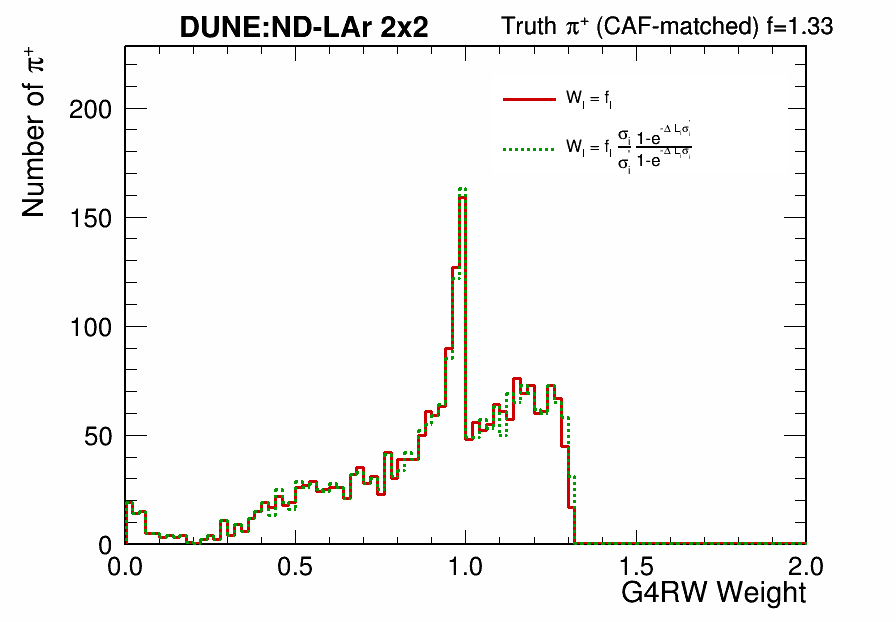
\includegraphics[scale=0.5]{fig02_eq310_comparison}
    \caption{G4RW weight distribution for CAF-matched truth \pip{} at
    $f = 1.33$, comparing $W_I = f_I$ (Eq.~\ref{eq:wi_old}) against
    $W_I$ as given by Eq.~\ref{eq:wi}. The shapes agree closely.}
    \label{fig:eq310_comparison}
\end{figure}

\subsection{\label{subsec:exclusive}Exclusive Channel Decomposition}

G4RW can scale the total inelastic cross section as a single number, or scale
individual exclusive channels. The latter requires knowing how \gfour{}
distributes inelastic interactions among final states as a function of momentum.
That information is supplied by the exclusive channel fraction files, referred
to throughout as fraction (aka "fracs") files.

For charged pions the channels are absorption (\texttt{abs}), charge exchange
(\texttt{cex}), double charge exchange (\texttt{dcex}), quasielastic scattering
(\texttt{inel}), and pion production (\texttt{prod}). The fractions are
dimensionless and normalized at every momentum point:
\begin{equation}
\label{eq:fracs_sum}
f_{\text{abs}}(p) + f_{\text{cex}}(p) + f_{\text{dcex}}(p)
+ f_{\text{inel}}(p) + f_{\text{prod}}(p) = 1 .
\end{equation}
The exclusive cross section for channel $c$ is recovered at runtime as
\begin{equation}
\label{eq:exclusive_xsec}
\sigma_c(p) = f_c(p)\,\sigma_I(p),
\end{equation}
where $\sigma_I(p)$ is the total inelastic term from \gfour{}'s internal tables.
The fracs file therefore stores only the decomposition, not the cross section
itself.

For nucleons the same scheme is used with channels defined by counting
outgoing nucleons: no outgoing nucleons (\texttt{0n0p}), one proton only
(\texttt{0n1p}), one neutron only (\texttt{1n0p}), one of each
(\texttt{1n1p}), and all remaining multi-nucleon topologies (\texttt{Other},
labelled \texttt{MnMp} in the figures). This decomposition is not part of
the standard distribution and was produced for this analysis, as presented in Section~\ref{subsec:fracs}.

The current analysis scales the total inelastic cross section rather than
individual channels; the fracs file is what would make per-channel
variation possible.

% ===========================================================================
\section{\label{sec:inputs}Required Inputs}
% ===========================================================================

Running G4RW requires three inputs: EDepSim files carrying full \gfour{}
trajectories, fracs files giving the exclusive channel decomposition, and a
FHiCL configuration file specifying what to vary and by how much. Each is
described below. The first two required work specific to this analysis.

\subsection{\label{subsec:edepsim_patch}EDepSim Files with Full Trajectories}

% \subsubsection{The trajectory granularity requirement}

G4RW evaluates Eq.~\ref{eq:ws} step by step, reading the position and momentum
at each \gfour{} transport step. EDepSim does not store them by default. Its \texttt{SelectTrajectoryPoints} routine, in
\texttt{EDepSimPersistencyManager.cc}, prunes trajectory points
geometrically, keeping points at volume boundaries and the track endpoints.
For G4RW this is not enough: a hadron crossing a uniform argon volume is
reduced to as few as two points, and the product over steps in
Eq.~\ref{eq:ws} collapses to as little as a single interval.

\subsubsection{The patch}

Throughout this note, \emph{patch} refers to the EDepSim sample produced
with full trajectory points retained, as distinguished from the default
\emph{unpatched} sample, in which \texttt{SelectTrajectoryPoints} prunes
most points away.
The fix is a bypass we inserted into \texttt{SelectTrajectoryPoints} ahead
of the pruning logic. For the species of interest, every stored trajectory
point is kept and the routine returns before the geometric pruning runs;
behaviour for all other particles is unchanged. The bypass condition is

\begin{bashcode}
if (std::abs(pdg) == 211 || pdg == 2212 ||
    pdg == 2112 || std::abs(pdg) == 321) {
    for (int i = 0; i < g4Traj->GetPointEntries(); ++i)
        selected.push_back(i);   // keep every step
    return;
}
\end{bashcode}

\noindent
covering $\pi^{\pm}$ ($\pm211$), protons (2212), neutrons (2112), and
$K^{\pm}$ ($\pm321$).


\subsubsection{Validation}

EDepSim was recompiled with this fix and used to regenerate the full
simulated 1000-file sample. A
diagnostic pass over the whole sample gives the trajectory point counts in
Table~\ref{tab:traj_points}. All six species show the full-trajectory signature.
The minimum of 2 points that appears for every species corresponds to tracks
that stop after a single step and is expected.

% SOURCE: slide 7 (trajectory points table)
\begin{table}[H]
\centering
\caption{Trajectory points per track in the patched sample.}
\setlength{\tabcolsep}{14pt}
\label{tab:traj_points}
\begin{tabular}{lcccc}
\hline\hline
Particle & PDG & Average points & Min & Max \\
\hline
$\pi^{+}$  & $+$211  & 47.3 & 2 & 1159 \\
$\pi^{-}$  & $-$211  & 44.2 & 2 & 1194 \\
proton     & $+$2212 & 9.1  & 2 & 7482 \\
neutron    & $+$2112 & 54.4 & 2 & 1080 \\
$K^{+}$    & $+$321  & 54.1 & 2 &  939 \\
$K^{-}$    & $-$321  & 50.5 & 2 &  869 \\
\hline\hline
\end{tabular}
\end{table}

Table~\ref{tab:traj_patch_dump} shows the effect on a single track. The
unpatched listing carries two points and one step of 6.83~cm; the patched
listing carries seven points resolving the same 6.83~cm into six steps, with the
momentum falling from 1180 to 1116~MeV along the way. The total path length is
unchanged, which is the expected behaviour: the patch changes only how finely
the trajectory is sampled.

% SOURCE: slide 7, "EDepSim Trajectory Patch for G4RW"
\begin{table}[H]
\centering
\caption{Stored trajectory points for a single $\pi^{+}$ track before
(Unpatched) and after (Patched), listing position, step length, momentum,
and \gfour{} process and subprocess codes at each point. The total path
length is 6.83~cm in both cases; the patch changes only how finely that
length is sampled.}
\label{tab:traj_patch_dump}
\setlength{\tabcolsep}{12pt}
\begin{tabular}{clrrrrrcc}
\hline\hline
\multicolumn{9}{c}{File=0000000 \quad Spill(entry)=3 \quad RunId=0 \quad EventId=3 \quad TrackId=6 \quad nPoints=7} \\ \\
\hline
& step & $x$ [mm] & $y$ [mm] & $z$ [mm] & $\Delta L$ [cm] & $|p|$ [MeV] & proc & subproc \\
\hline
\multirow{2}{*}{Unpatched}
& 0 & $-$1006.6 & 1167.6 & 2723.6 & 0.00 & 1180.2 & 2 & 22 \\
& 1 & $-$1004.8 & 1152.6 & 2790.2 & 6.83 & 0.0    & 4 & 121 \\
\hline
\multirow{7}{*}{Patched}
& 0 & $-$1006.6 & 1167.6 & 2723.6 & 0.00 & 1180.2 & 2 & 22 \\
& 1 & $-$1006.0 & 1163.5 & 2742.3 & 1.92 & 1158.2 & 2 & 2 \\
& 2 & $-$1005.8 & 1161.4 & 2751.6 & 0.95 & 1149.4 & 1 & 91 \\
& 3 & $-$1005.6 & 1159.4 & 2760.2 & 0.89 & 1149.4 & 1 & 91 \\
& 4 & $-$1005.1 & 1155.2 & 2778.8 & 1.90 & 1123.7 & 2 & 2 \\
& 5 & $-$1005.0 & 1154.6 & 2781.3 & 0.26 & 1115.9 & 2 & 2 \\
& 6 & $-$1004.8 & 1152.6 & 2790.2 & 0.91 & 0.0    & 4 & 121 \\
\hline\hline
\end{tabular}
\end{table}

% SOURCE: slide 7, "EDepSim Trajectory Patch for G4RW"
% \begin{figure}[H]
%     \centering
%     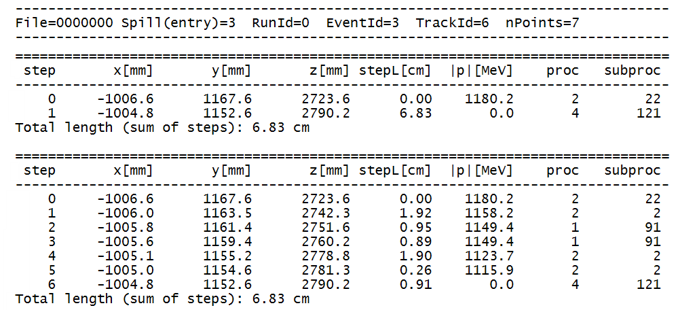
\includegraphics[width=0.92\textwidth]{fig03_traj_patch_dump}
%     \caption{Stored trajectory points for a single $\pi^{+}$ track
%     before (top) and after (bottom) the patch, listing position, step length,
%     momentum, and \gfour{} process and subprocess codes at each point. The
%     unpatched track carries two points and a single 6.83~cm step; the patched
%     track resolves the same path into six steps.}
%     \label{fig:traj_patch_dump}
% \end{figure}

% Patching does not inflate the output: a hadded patched sample and the
% corresponding unpatched MiniRun5 sample are comparable in size
% ($\sim$460~MB versus $\sim$489~MB for the same file set).

\subsubsection{\label{subsec:sample_choice}Choice of EDepSim sample}

The EDepSim sample used for weight production must satisfy three conditions at
once: it must reproduce the track lengths seen in the CAF, its event numbering
must match the CAF interaction identifier, and it must carry full trajectories.
Five candidate samples were compared --- the official MiniRun5 production plus
four produced at Argonne --- differing in geometry
(\texttt{Merged2x2MINERvA\_v4\_withRock} versus \texttt{Merged2x2MINERvA\_v4\_noRock}), patch
status, and GENIE input set. Their properties are summarised in
Table~\ref{tab:edepsim_samples}.

\begin{table}[H]
\centering
\caption{EDepSim samples compared for G4RW weight production. All ANL samples
use only \texttt{genie.nu} GTRAC files (argon interactions); the official sample
additionally includes \texttt{genie.rock}. ``Patched'' refers to preservation of
intermediate \gfour{} trajectory points.}
\label{tab:edepsim_samples}
\setlength{\tabcolsep}{14pt}
\begin{tabular}{cl|cccc}
\hline\hline
\# & Sample & Geometry & Patched & GENIE input & Matches CAF \\
\hline
1 & Official unpatched & \texttt{withRock} & No  & \texttt{nu} + \texttt{rock} & Yes \\
2 & ANL unpatched      & \texttt{noRock}   & No  & \texttt{nu} only            & No  \\
3 & ANL patched        & \texttt{noRock}   & Yes & \texttt{nu} only            & No  \\
4 & ANL unpatched      & \texttt{withRock} & No  & \texttt{nu} only            & Yes \\
5 & ANL patched        & \texttt{withRock} & Yes & \texttt{nu} only            & Yes \\
\hline\hline
\end{tabular}
\end{table}

The geometry choice determines where a hadron's trajectory ends: in
\texttt{withRock}, a hadron leaving the argon immediately enters rock and
interacts there, consistent with the CAF; in \texttt{noRock}, the
surrounding material is vacuum, so the same hadron travels considerably
further before interacting, which is why the \texttt{noRock} samples fail
to match the CAF. Sample 5 (\texttt{patched\_withRock\_genieNu}) is the
only one satisfying all three conditions and is used for all weight
production reported here.

A fraction of CAF hadrons originate in the upstream rock rather than in
argon. These are present in the official sample but absent from the ANL
samples, which use \texttt{genie.nu} only. They have no entry in the weight
files, receive the default weight $w = 1.0$, and contribute no systematic
shift --- the correct treatment, since they are not argon interactions.


\subsection{\label{subsec:fracs}Exclusive Channel Fraction Files}

The fracs file supplies the channel fraction $f_c(p)$ of
Eq.~\ref{eq:exclusive_xsec}, the fraction of the total inelastic cross
section carried by channel $c$ at momentum $p$, one object per channel.
The standard \texttt{dune\_pardata} distribution~\cite{dune_pardata}
provides a full five-channel decomposition for \pip{}, covering
11--9001~MeV/$c$; this file is used unmodified. We generated fracs files for \pim{}, protons, and neutrons using the
\texttt{G4Cascade} application, extending to the same upper momentum of
9001~MeV/$c$. A hadron with momentum above this range has no
per-channel decomposition available and receives a weight of $w = 1.00$;
%Section~\ref{subsec:two_trends} shows this directly in the reconstructed sample. This range is sufficient for the samples considered here. 
Figure~\ref{fig:fracs_all_species} shows the exclusive channel fractions for all four species.

% SOURCE: slide 3, "How Geant4 Tracks Particles, and Where G4RW Comes In"
\begin{figure}[htb!]
    \centering
    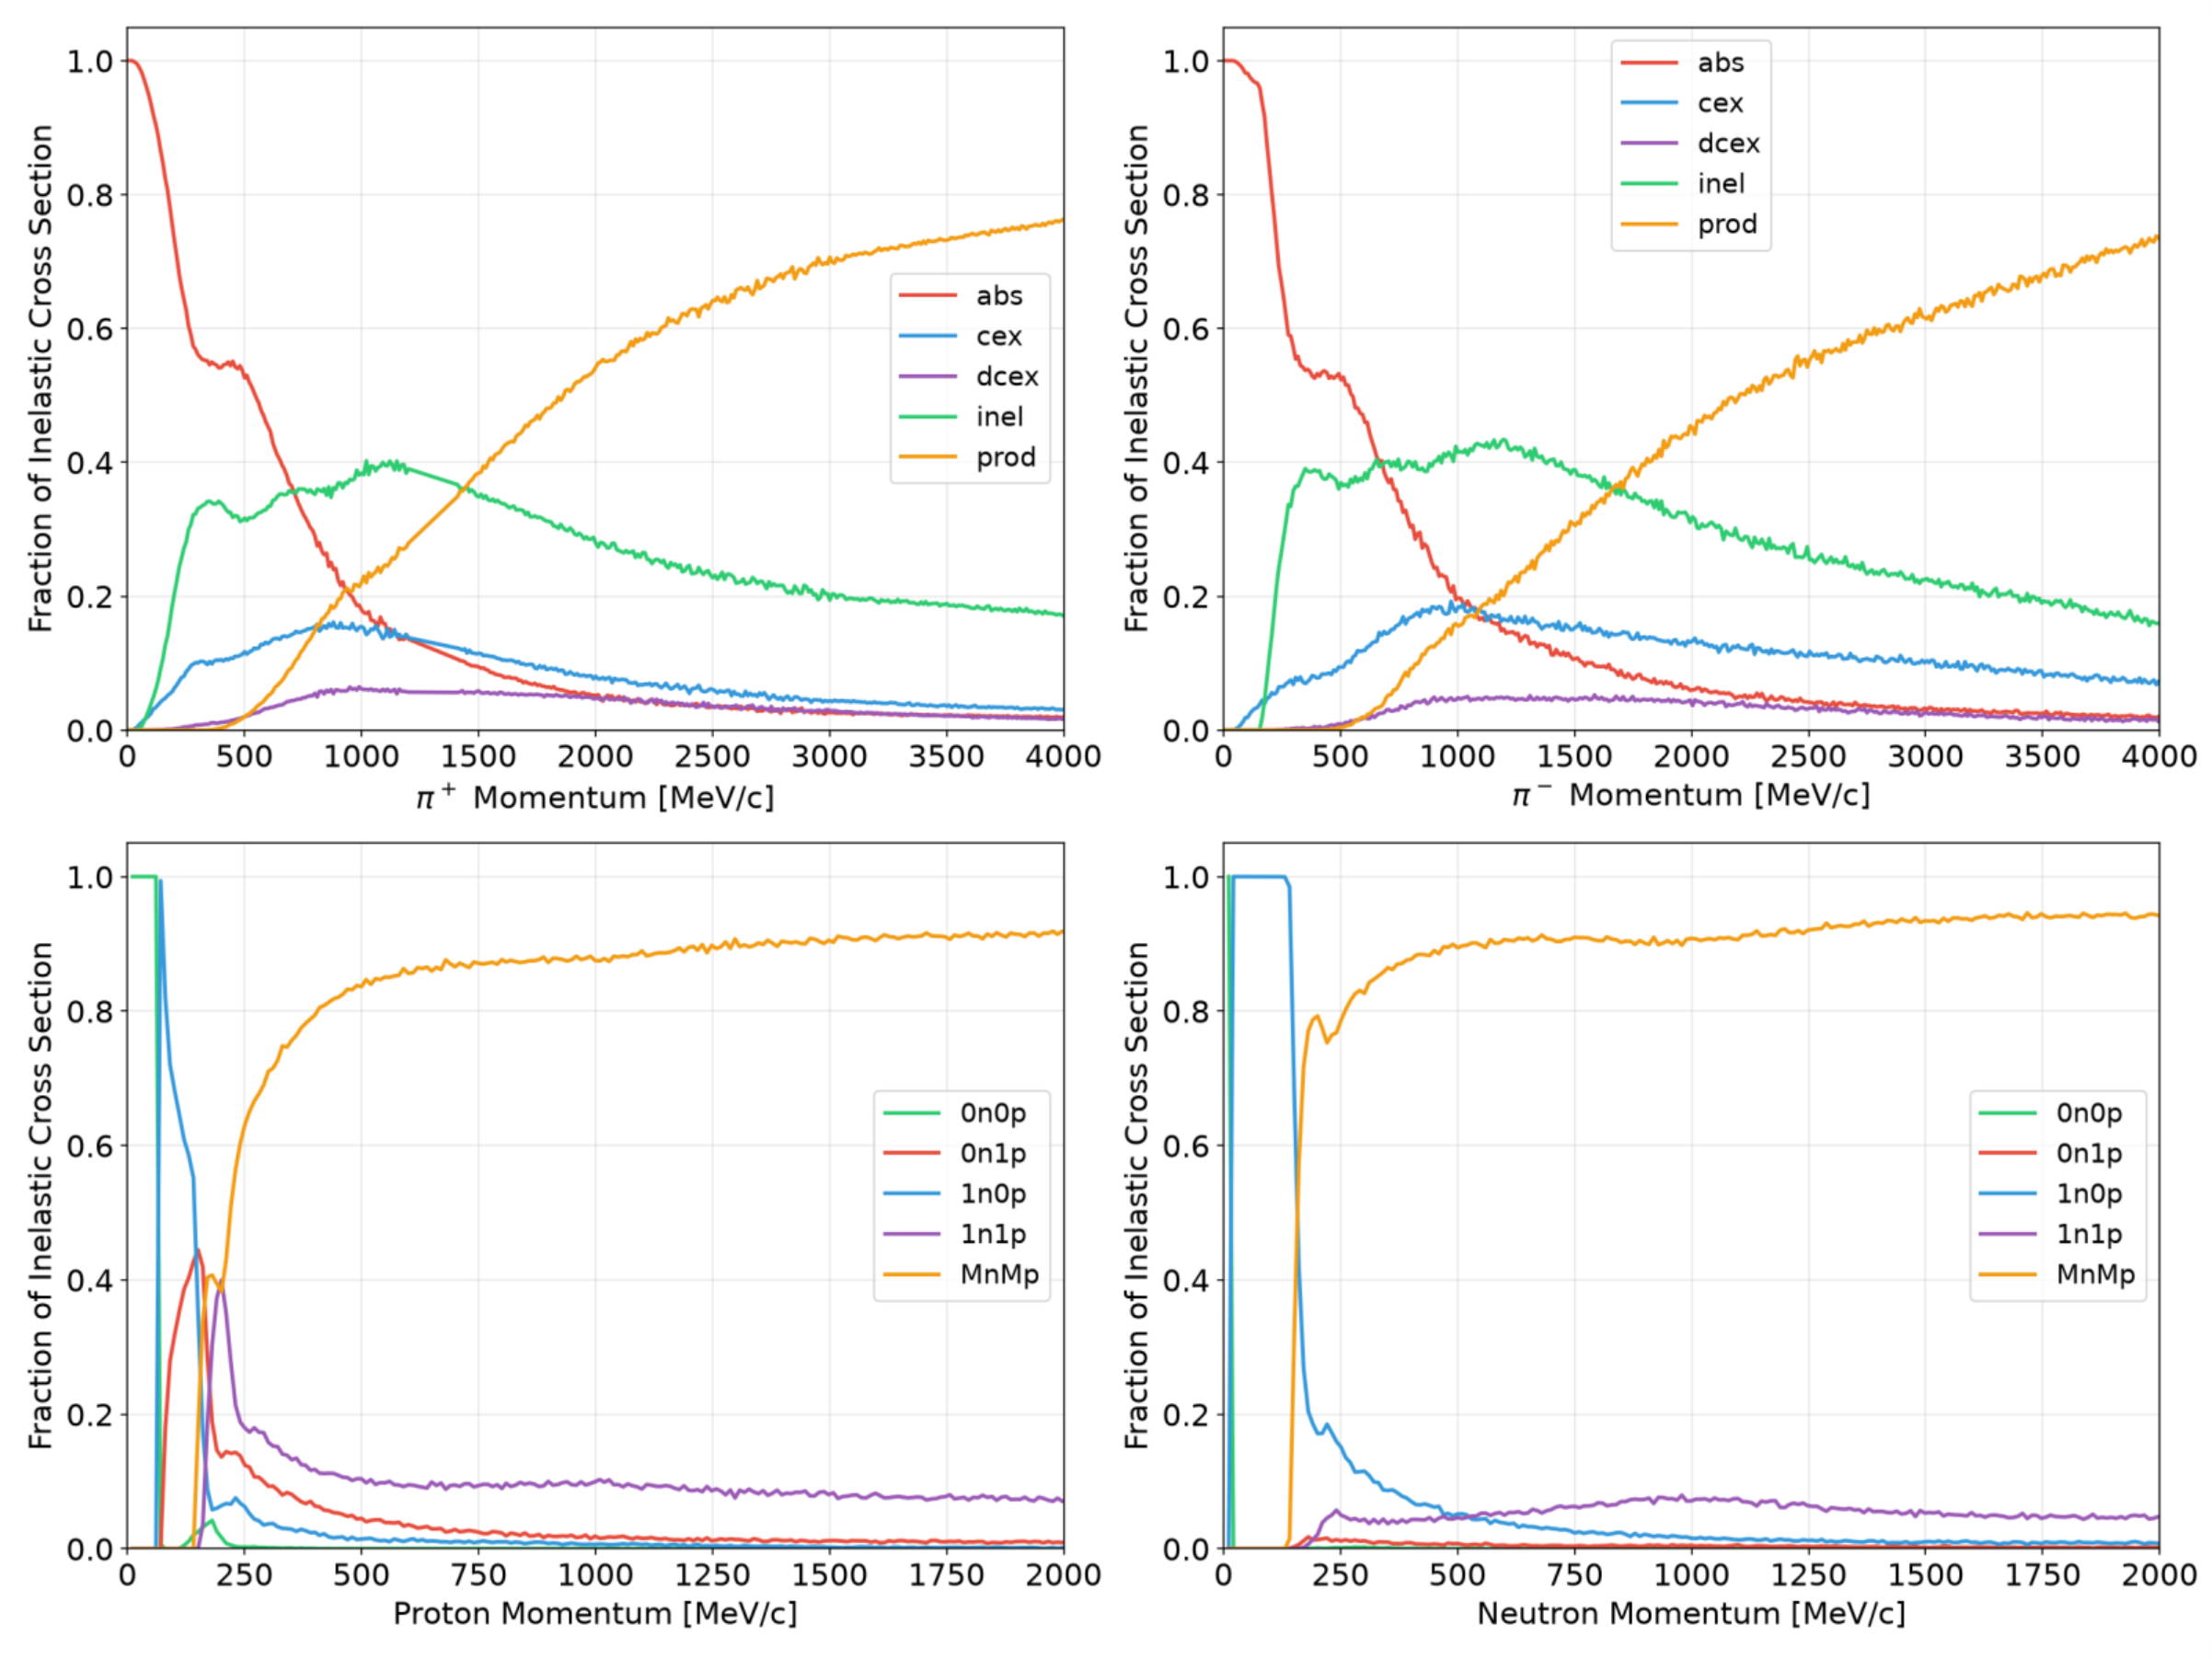
\includegraphics[width=0.94\textwidth]{fig04_fracs_all_species}
    \caption{Exclusive channel fractions as a function of momentum in
    liquid argon, computed with \texttt{G4Cascade} by firing $10,000$ particles
    into argon at each momentum point and classifying the outgoing final state.
    Top: $\pi^{+}$ (left, official \texttt{dune\_pardata} file) and $\pi^{-}$
    (right, generated at ANL), with channels \texttt{abs}, \texttt{cex},
    \texttt{dcex}, \texttt{inel}, \texttt{prod}. Bottom: proton (left) and
    neutron (right), both generated at ANL, with nucleon-counting channels
    \texttt{0n0p}, \texttt{0n1p}, \texttt{1n0p}, \texttt{1n1p}, and
    \texttt{MnMp}. Fractions sum to unity at every momentum point in all four
    cases. For visual clarity, the plotted momentum range is truncated below
    the full fracs-file range of 11--9001~MeV/$c$: pions are drawn up to
    4000~MeV/$c$ and protons and neutrons up to 2000~MeV/$c$.}
    \label{fig:fracs_all_species}
\end{figure}


To produce fracs files, \texttt{G4Cascade} fires $10,000$ particles into a liquid argon target at
each of a set of momentum points, classifies the final state of each
inelastic interaction, and writes the resulting channel fractions. The neutron configuration is shown below; the
proton case differs only in \texttt{Type} and \texttt{Outfile}, and the
$\pi^{-}$ case additionally sets \texttt{NPi0\_Cex: true} with 150~MeV
thresholds on charged pion secondaries, matching the settings used for the
official $\pi^{+}$ file so the two are directly comparable.

\begin{bashcode}
#include "g4rw_material.fcl"
#include "g4rw_physlist.fcl"
Type:       2112
NCascades:  10000
Range:      [11., 9001.]
NDivisions: 880
Outfile:    ".../G4RW/G4Cascade/LAr_N_cascade_0_9000.root"
Material:   @local::LAr
NPi0_Cex:   false
Thresholds: []
Physlist:   @local::Physlist_default
\end{bashcode}


\subsection{\label{subsec:fcl}FHiCL Configuration}

The FHiCL file tells G4RW what to vary. It specifies the target material, the
path to the fracs file, the overall scale factor (\texttt{Weight}), and a
\texttt{ParameterSet} listing the channels to vary. Each entry in the
\texttt{ParameterSet} carries the channel name (\texttt{Cut}), the momentum
range over which the variation applies (\texttt{Range}), the nominal value
(always 1.0, since a scale factor of 1
reproduces the unmodified \gfour{} cross section), and the prior width (\texttt{Sigma}). A sample \pip{} configuration
is shown below.

\begin{bashcode}
Weight: 0.67
Material: {
  Name: "liquidArgon"
  Density: 1.400
  Components: [
    { Z: 18
      Mass: 39.948
      Fraction: 1. }
  ]
}
FracsFile: "Geant4ReweightInput/LAr_PiPlus_cascade_0_9000.root"
ParameterSet: [
  { Cut: "reac"
    Name: "fReac"
    Range: [0., 2000.]
    Nominal: 1.0
    Sigma: 0.67 }
]
\end{bashcode}

\noindent
The single \texttt{Cut: "reac"} entry scales the total inelastic cross
section, and is the only cross section varied; with no \texttt{Cut:
"elast"} entry present, $\sigma'_E = \sigma_E$ and the elastic
contributions cancel in Eq.~\ref{eq:ws}.

\noindent
The single \texttt{Cut: "reac"} entry scales the total inelastic cross
section, and is the only cross section varied; with no \texttt{Cut:
"elast"} entry present, $\sigma'_E = \sigma_E$ and the elastic
contributions cancel in Eq.~\ref{eq:ws}.

The scale factor's prior follows the parameterization described in
Refs.~\cite{calcutt_thesis,pinzon_guerra}: a $\pm33\%$ width around the
nominal value of 1.0, giving 0.67 as the downward variation
and 1.33 as the upward one. This width was adopted for current studies,
motivated by the spread between \gfour{} predictions and external $\pi$--$A$
scattering data, shown in Figure~\ref{fig:pion_data_spread}.


% SOURCE: slide 4, "Producing G4RW Weights: Scale Factor Choice"
\begin{figure}[htb!]
    \centering
    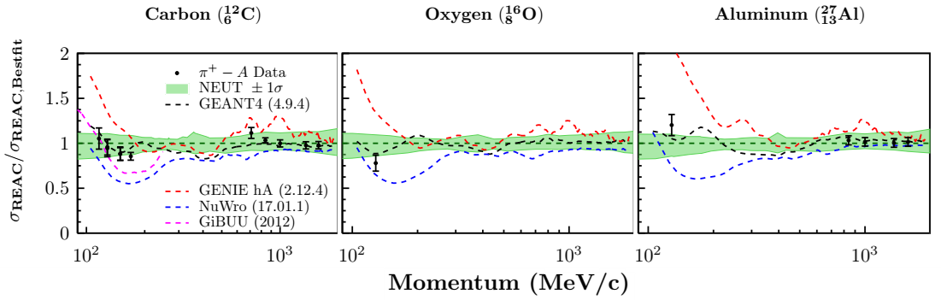
\includegraphics[width=0.95\textwidth]{fig05_pion_data_spread}
    \caption{Ratio of the reactive cross section to its best-fit
    value for $\pi^{+}$ on carbon, oxygen, and aluminium, comparing external
    scattering data against \gfour{} and several neutrino-generator cascade
    models, from Ref.~\protect\cite{pinzon_guerra}. The spread between models at
    a given momentum is what motivates the $\pm33\%$ prior adopted here for
    argon.}
    \label{fig:pion_data_spread}
\end{figure}

% ===========================================================================
\section{\label{sec:species}Extending G4RW to Six Hadron Species}
% ===========================================================================

Extending G4RW to the species relevant for the $2\times2$ and ND-LAr touched three
largely independent components: the EDepSim trajectory patch, which
determines whether a species has usable trajectories at all (Section~\ref{subsec:edepsim_patch}); the fracs file, which
supplies the channel decomposition (Section~\ref{subsec:fracs}); and the \texttt{Geant4Reweight} source,
which determines whether a species has a reweighter class with exclusive
channels (Section~\ref{subsec:code_changes}). A fourth
component, the $2\times2$ weight-production executables and their FHiCL
configurations, is what actually produces weight files (Section~\ref{sec:weights}).
Table~\ref{tab:species_status} gives the state of each hadron species
across each of these components.


% SOURCE: slide 2 (status sentence; not a slide table)
\begin{table}[H]
\centering
\caption{Coverage by species and by component. ``Native'' means the
capability was already present in the distributed framework and required no
change here. ``Weight production'' refers to the component that produces
per-particle weight trees. Kaons carry the EDepSim patch as groundwork only, so
that trajectories exist if kaon reweighting is taken up later.}
\label{tab:species_status}
\setlength{\tabcolsep}{12pt}
\begin{tabular}{lcccc}
\hline\hline
Species & EDepSim patch & G4RW code & Fracs file & Weight production \\
\hline
$\pi^{+}$ & Added   & Native      & Native (\texttt{dune\_pardata}) & Done \\
$\pi^{-}$ & Added   & Native      & Generated at ANL                  & Done \\
proton    & Added   & Modified    & Generated at ANL                  & Done \\
neutron   & Added    & Modified    & Generated at ANL                  & Done \\
%$K^{+}$   & Added    & Not started & Not started                     & Not started \\
%$K^{-}$   & Added    & Not started & Not started                     & Not started \\
$K^{+}$   & Added    & TBD & TBD                     & TBD \\
$K^{-}$   & Added    & TBD & TBD                     & TBD \\
\hline\hline
\end{tabular}
\end{table}

% --------------------------------------------------------------------------
%
% ---------------------------------------------------------------------------

\subsection{\label{subsec:code_changes}\texttt{Geant4Reweight} Source Changes}

Giving nucleons an exclusive channel decomposition required modifying two
source files. Both changes mirror a pattern already present for pions. 
The $\pi^{-}$ required no source changes at all, since
\texttt{G4PiMinusReweighter.cc} already implements all five exclusive
channels natively.

\paragraph{Reweighter classes.} The \texttt{G4ProtonReweighter.cc} and
\texttt{G4NeutronReweighter.cc} were each changed in two places. The constructor
channel list was changed from the single placeholder channel to the five
nucleon-counting channels:

\begin{cppcode}
// before
: G4Reweighter(..., {"total"}, ...)
// after
: G4Reweighter(..., {"0n0p", "0n1p", "1n0p", "1n1p", "Other"}, ...)
\end{cppcode}

\noindent
and \texttt{GetInteractionSubtype()}, which returned a hardcoded string, was
replaced by logic that classifies each inelastic interaction by counting
secondary nucleons:

\begin{cppcode}
std::string G4NeutronReweighter::GetInteractionSubtype(
    const G4ReweightTraj & theTraj) {
  int nProtons  = theTraj.HasChild(2212).size();
  int nNeutrons = theTraj.HasChild(2112).size();
  if      (nNeutrons == 0 && nProtons == 0) return "0n0p";
  else if (nNeutrons == 0 && nProtons == 1) return "0n1p";
  else if (nNeutrons == 1 && nProtons == 0) return "1n0p";
  else if (nNeutrons == 1 && nProtons == 1) return "1n1p";
  else                                      return "Other";
}
\end{cppcode}

\noindent
The proton version is identical apart from the class name. 
% This mirrors
% \texttt{G4PiPlusReweighter::GetInteractionSubtype()}, which classifies by
% counting outgoing pions.

\paragraph{Parameter maker.} \texttt{G4ReweightParameterMaker.cc} defines which
channel names are accepted for each species. The proton (2212) and neutron
(2112) cases were changed from \texttt{\{"total", "reac"\}} to the five
exclusive channels plus \texttt{"reac"}. Retaining \texttt{reac} is necessary:
it is the parameter used when scaling the total inelastic cross section.


% ===========================================================================
\section{\label{sec:weights}Weight Production and Validation}
% ===========================================================================

\subsection{\label{subsec:executable}Scale Factors and the Weight-Production Executable}

Although the SI cross-section channels and its scale factors are implemented as independent, the current production varies all cross-section channels by a same scale factor. The five SI cross-section variations are performed, using the following scale factors applied in each of five single passes over each file:
\begin{equation}
\label{eq:scale_factors}
f \in \{0.34,\; 0.67,\; 1.33,\; 1.66,\; 2.00\}.
\end{equation}
The $\pm33\%$ pair ($f = 0.67, 1.33$) is the physically motivated one
(Section~\ref{subsec:fcl}). The remaining three ($f = 0.34, 1.66, 2.00$,
corresponding to $\pm66\%$ and $+100\%$) are included to exercise the
machinery across a wider range.

Weights are produced by a C++ executable that
runs over the patched EDepSim trajectories, computes the per-track G4RW
weight for each of the five scale factors, and writes the result to a
\texttt{TTree} named \texttt{g4rwEvt} with one entry per weighted particle,
carrying the identifiers needed to match a weight back to a reconstructed
particle (see Table~\ref{tab:weight_tree}).

\begin{table}[H]
\centering
\caption{Branches of the \texttt{g4rwEvt} output tree.}
\label{tab:weight_tree}
\setlength{\tabcolsep}{14pt}
\begin{tabular}{lll}
\hline\hline
Branch & Type & Meaning \\
\hline
\texttt{file\_idx} & \texttt{int}    & File index parsed from the input filename \\
\texttt{spill\_id} & \texttt{int}    & EDepSim spill index \\
\texttt{run\_id}   & \texttt{int}    & EDepSim \texttt{RunId} \\
\texttt{event\_id} & \texttt{int}    & $\texttt{RunId}\times10^{6} + \texttt{EventId}$ \\
\texttt{track\_id} & \texttt{int}    & \gfour{} track ID \\
\texttt{pdg}       & \texttt{int}    & PDG code of the reweighted particle \\
\texttt{weight}    & \texttt{double} & G4RW weight, one branch per scale factor \\
\texttt{len}       & \texttt{double} & Total track length (cm) \\
\hline\hline
\end{tabular}
\end{table}

\subsection{\label{subsec:single_track}Single-Track Validation}

Before looking at distributions, it is worth following an example where the machinery is applied on a single
track, where every step can be inspected. Figure~\ref{fig:single_track} does
this for a $\pi^{+}$ with 45 recorded trajectory points spanning 14.4~cm and
ending in a hadron-inelastic interaction.

% SOURCE: slide 9, "Single-Track Test: Weight vs. Track Length"
\begin{figure}[htb!]
    \centering
    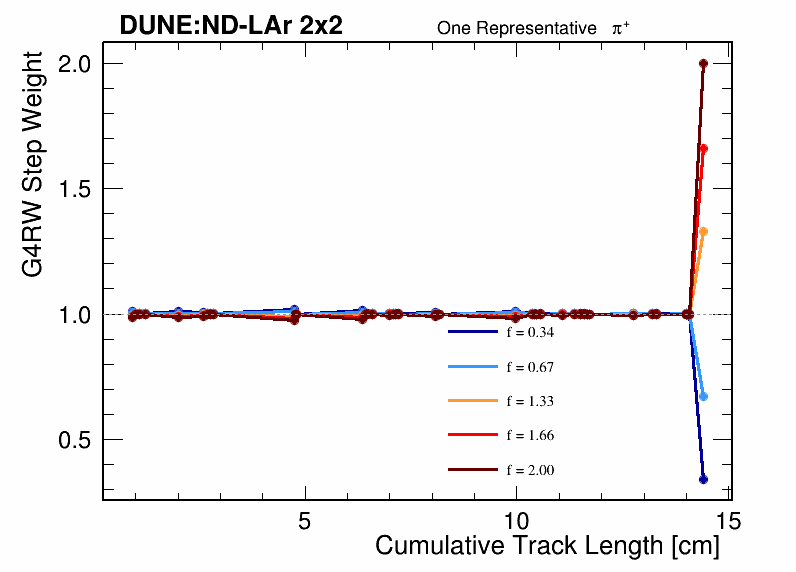
\includegraphics[width=0.48\textwidth]{fig06a_step_weight}\hfill
    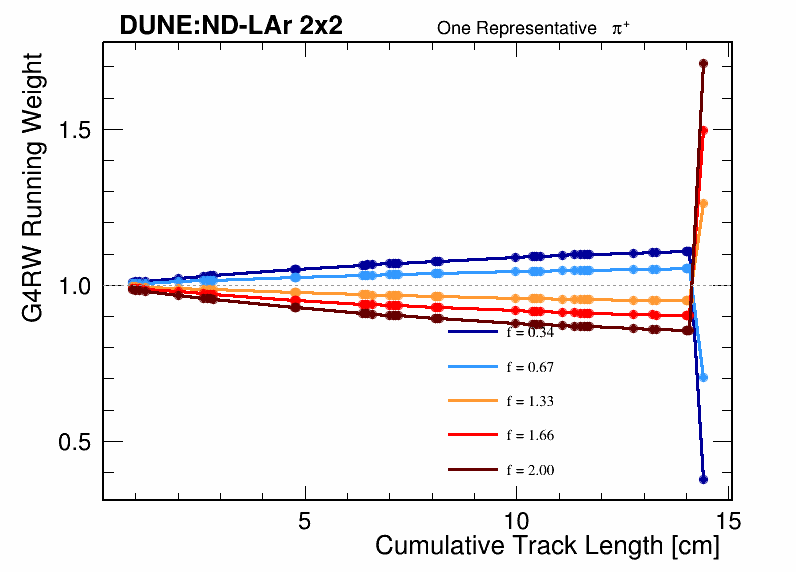
\includegraphics[width=0.48\textwidth]{fig06b_running_weight}
    \caption{Per-step weight (left) and cumulative running weight
    (right) along a single $\pi^{+}$ track of 45 trajectory points and 14.4~cm,
    for each of the five scale factors. The per-step weight stays close to unity
    at every non-interacting step, because a step length is a small fraction of
    the mean free path. The final step carries the interaction term of
    Eq.~\ref{eq:wi} and is not constrained to lie near unity, which produces the
    sharp excursion at the end of the track.}
    \label{fig:single_track}
\end{figure}

The shape explains a feature that recurs throughout the distributions below. At
every non-interacting step the survival ratio of Eq.~\ref{eq:ws} deviates from
unity only slightly, because $\Delta L_i \sigma_i$ is small. For $f < 1$ survival
is slightly \emph{more} likely at each step, so the running weight drifts above
unity along the track; for $f > 1$ it drifts below. The final step then applies
the interaction term, which scales with $f$ itself and pulls the weight in the
opposite direction. The curves therefore cross near the end of the track.

\subsubsection{\label{subsec:hand_check}Verifying the final step by hand}

Table~\ref{tab:hand_check} works through the final step of that track
explicitly, and reproduces the saved production weight. This is the check that
confirms the Eq.~\ref{eq:wi} implementation described in
Section~\ref{subsec:eq310} is correct.

% SOURCE: slide 10, "Verifying the Final Weight by Hand: Example 2"
\begin{table}[H]
\centering
\caption{Hand evaluation of Eq.~\ref{eq:wi} at the final step of the
track in Figure~\ref{fig:single_track} (File 0000000, RunId 0, EventId 7,
TrackId 3, PDG 211), at $f = 1.33$. The result reproduces the saved production
weight.}
\label{tab:hand_check}
\setlength{\tabcolsep}{18pt}
\begin{tabular}{ll}
\hline\hline
Quantity & Value \\
\hline
Running weight after 44 steps, $W_S$      & 0.950046 \\
Last step length, $\Delta L_{45}$          & 0.345925 cm \\
$\sigma_I^{\text{nom}}$ at last step ($p \approx 84.84$ MeV/$c$)
                                           & 0.003982 cm$^{-1}$ \\
$\sigma_I'$ at last step $= f\,\sigma_I^{\text{nom}}$
                                           & $1.33 \times 0.003982 = 0.005296$ cm$^{-1}$ \\
$\sigma_E^{\text{nom}}$ at last step        & 0.002484 cm$^{-1}$ \\
$\sigma = \sigma_I + \sigma_E$              & $0.003982 + 0.002484 = 0.006466$ cm$^{-1}$ \\
$\sigma' = \sigma_I' + \sigma_E$            & $0.005296 + 0.002484 = 0.007780$ cm$^{-1}$ \\
$W_I$ (Eq.~\ref{eq:wi})                     & $1.33 \times \frac{0.006466}{0.007780}
                                               \times \frac{0.00268766}{0.002234219}
                                               = 1.329698$ \\
Final weight                                & $0.950046 \times 1.329698 = 1.263274$ \\
\hline\hline
\end{tabular}
\end{table}

% For comparison, the distributed implementation returns $1.262987$ for the same
% track, differing in the fourth decimal place. The size of the shift is consistent
% with the $-\Delta/2$ estimate of Section~\ref{subsec:eq310}.

\iffalse
\subsubsection{\label{subsec:patched_unpatched}Patched against unpatched
trajectories}

The trajectory patch changes the weight by changing how finely the survival
product is sampled. How much it matters depends on how much the momentum changes
along the track, which is what the two examples below are chosen to contrast.

Example 1 is a track of 6.83~cm whose momentum falls only from 1180 to
1116~MeV/$c$, a change of about $5.6\%$. Patched, it carries six steps; unpatched,
one. Example 2 is the 14.4~cm track of Figure~\ref{fig:single_track}, whose
momentum falls from 179 to 85~MeV/$c$, a change of about $53\%$; patched it
carries 45 steps against 4 unpatched. Tables~\ref{tab:example1} and
\ref{tab:example2} give the weights.

% SOURCE: slide 26, Example 1 weights table
\begin{table}[H]
\centering
\caption{Example 1. Weights for a $\pi^{+}$ track of 6.83~cm over which
the momentum falls by about $5.6\%$, comparing patched (6 steps) and unpatched
(1 step) trajectories. The $f = 1.00$ row is a sanity check: the weight is
exactly unity for both.}
\label{tab:example1}
\begin{tabular}{cccc}
\hline\hline
Scale factor & Patched $w$ & Unpatched $w$ & Difference \\
\hline
1.00 & 1.000000 & 1.000000 & 0\% (sanity check) \\
0.34 & 0.360144 & 0.360101 & 0.012\% \\
0.67 & 0.689562 & 0.689521 & 0.006\% \\
1.33 & 1.292270 & 1.292346 & 0.006\% \\
1.66 & 1.567152 & 1.567338 & 0.012\% \\
2.00 & 1.832972 & 1.833301 & 0.018\% \\
\hline\hline
\end{tabular}
\end{table}

% SOURCE: slide 28, Example 2 weights table
\begin{table}[H]
\centering
\caption{Example 2. Weights for a $\pi^{+}$ track of 14.4~cm over which
the momentum falls by about $53\%$, comparing patched (45 steps) and unpatched
(4 steps) trajectories. The patched-unpatched difference is roughly two orders
of magnitude larger than in Table~\ref{tab:example1}.}
\label{tab:example2}
\begin{tabular}{cccc}
\hline\hline
Scale factor & Patched $w$ & Unpatched $w$ & Difference \\
\hline
1.00 & 1.000000 & 1.000000 & 0\% (sanity check) \\
0.34 & 0.377047 & 0.381134 & 1.1\% \\
0.67 & 0.705559 & 0.709372 & 0.5\% \\
1.33 & 1.262971 & 1.256181 & 0.5\% \\
1.66 & 1.496895 & 1.480844 & 1.1\% \\
2.00 & 1.709915 & 1.682211 & 1.6\% \\
\hline\hline
\end{tabular}
\end{table}

The comparison isolates what the patch does. An unpatched trajectory evaluates
the cross section at a single momentum and assumes it holds over the whole
track. When the momentum barely changes, that assumption costs almost nothing,
and the two agree to better than $0.02\%$. When the momentum falls by half, the
cross section at the start of the track is not representative of the cross
section at the end, and the disagreement grows to $1.6\%$. The effect is
therefore bounded by how much a track slows down, not by its length as such.

% SOURCE: slide 27, "Single-Track Test: Running Weight, Patched vs. Unpatched (Example 1) [Contd.]"
\begin{figure}[H]
    \centering
    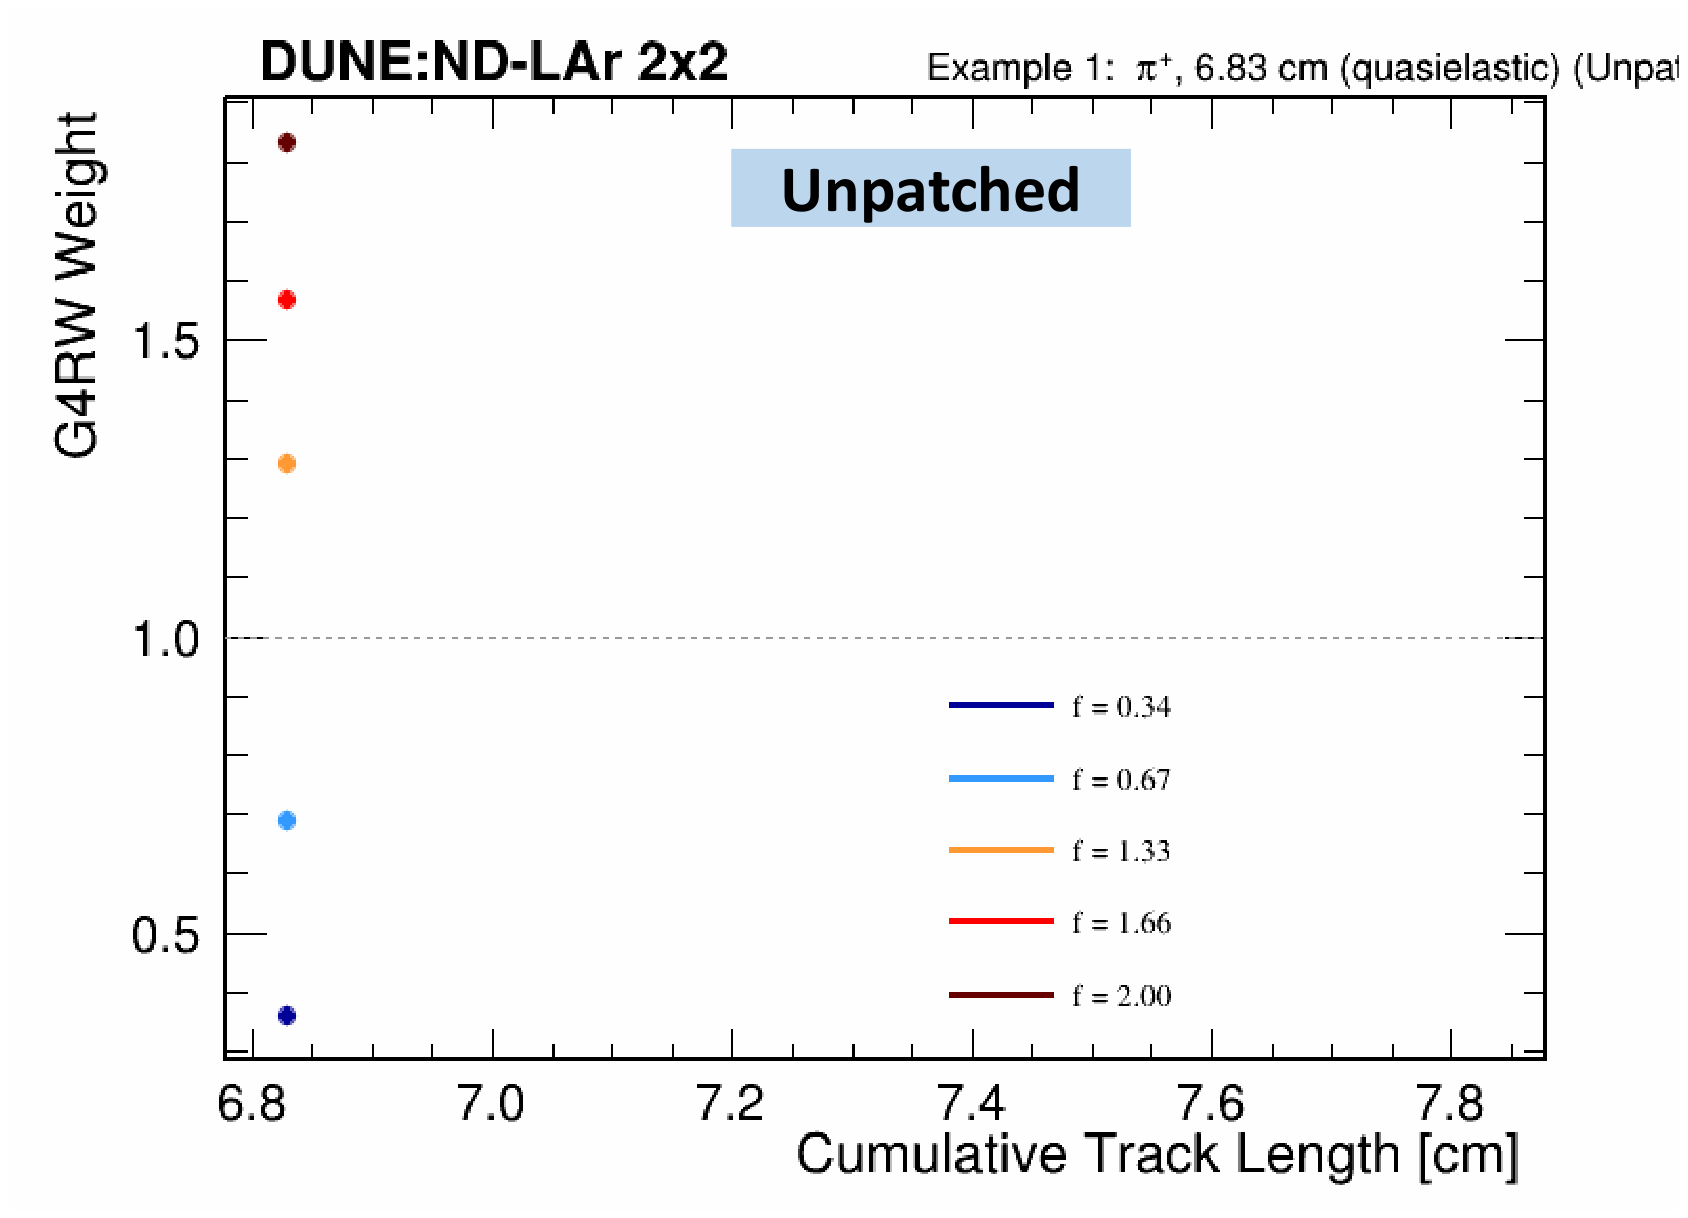
\includegraphics[width=0.48\textwidth]{fig07a_ex1_unpatched}\hfill
    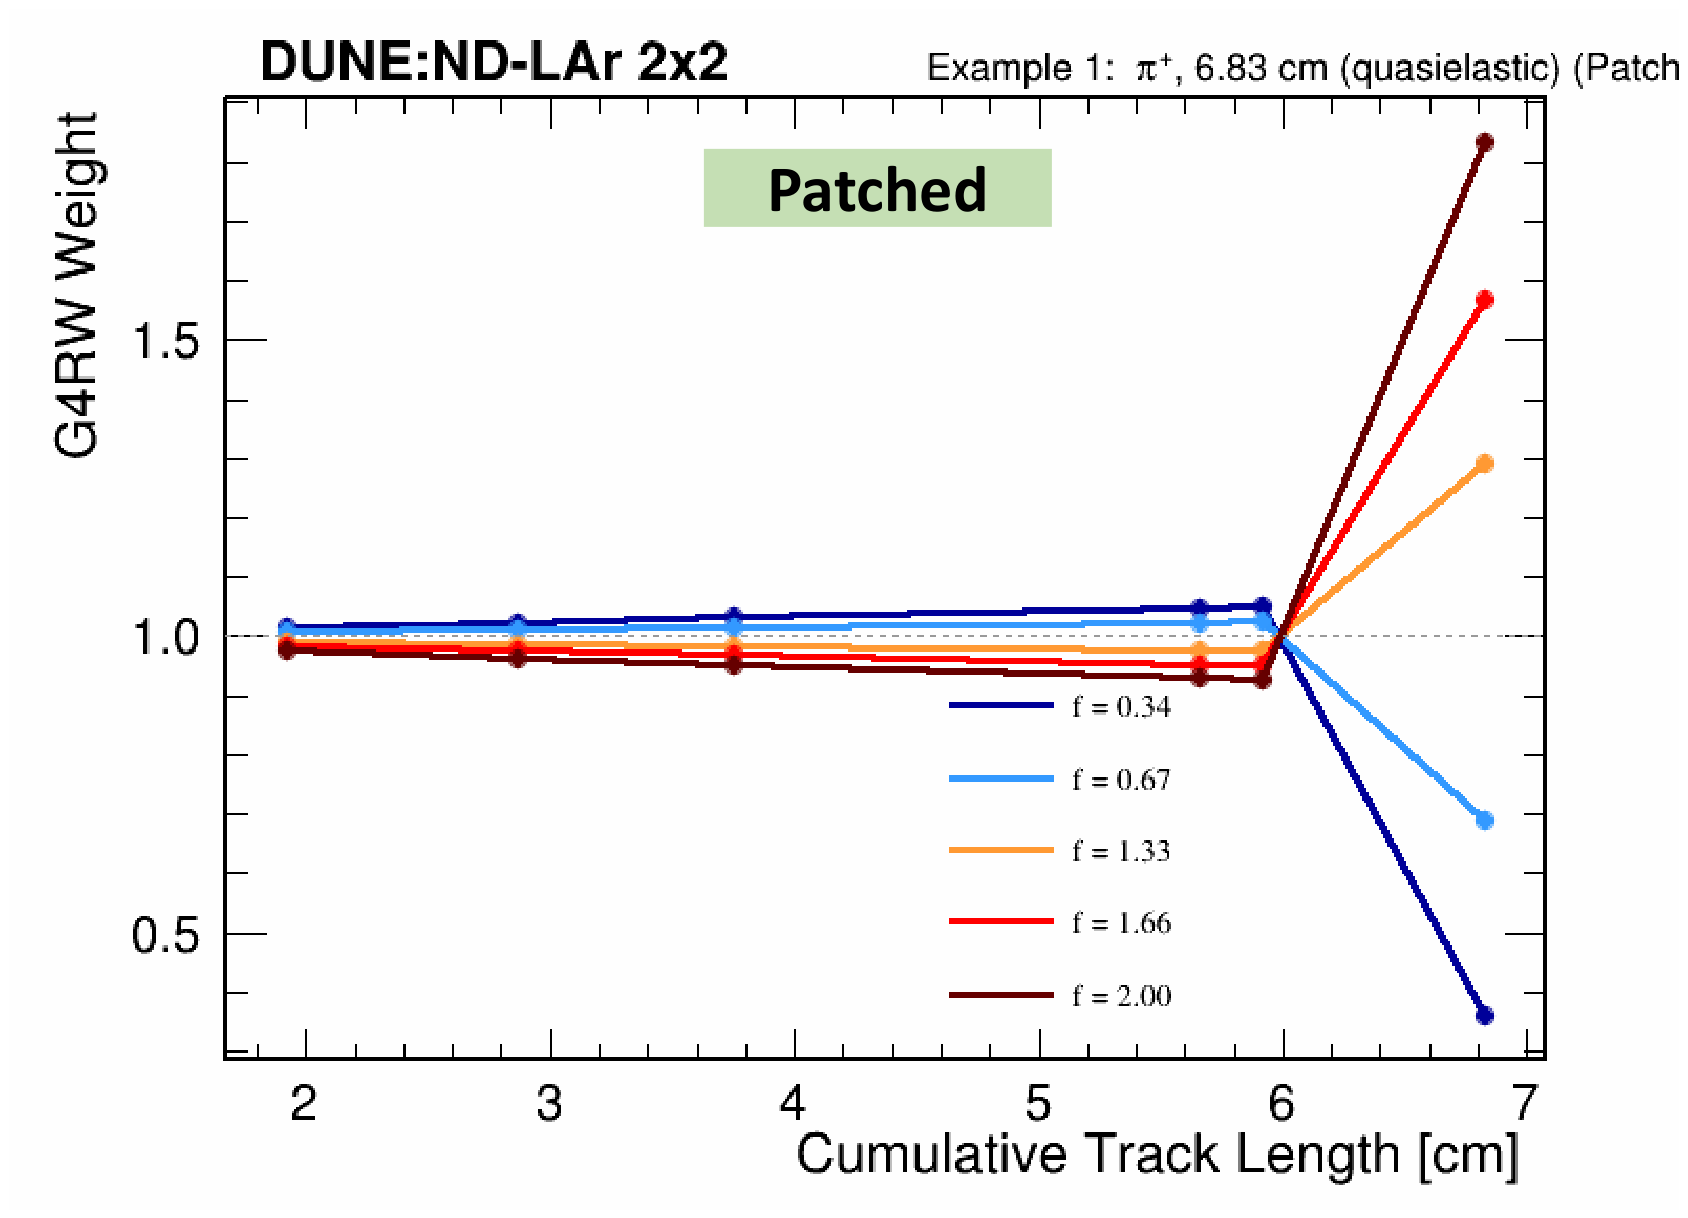
\includegraphics[width=0.48\textwidth]{fig07b_ex1_patched}
    \caption{Running weight against cumulative track length for
    Example 1, unpatched (left, one step) and patched (right, six steps), for
    each of the five scale factors. With only a single recorded step the
    unpatched case has no intermediate structure to show.}
    \label{fig:example1_running}
\end{figure}

% SOURCE: slide 29, "Single-Track Test: Running Weight, Patched vs. Unpatched (Example 2) [Contd.]"
\begin{figure}[H]
    \centering
    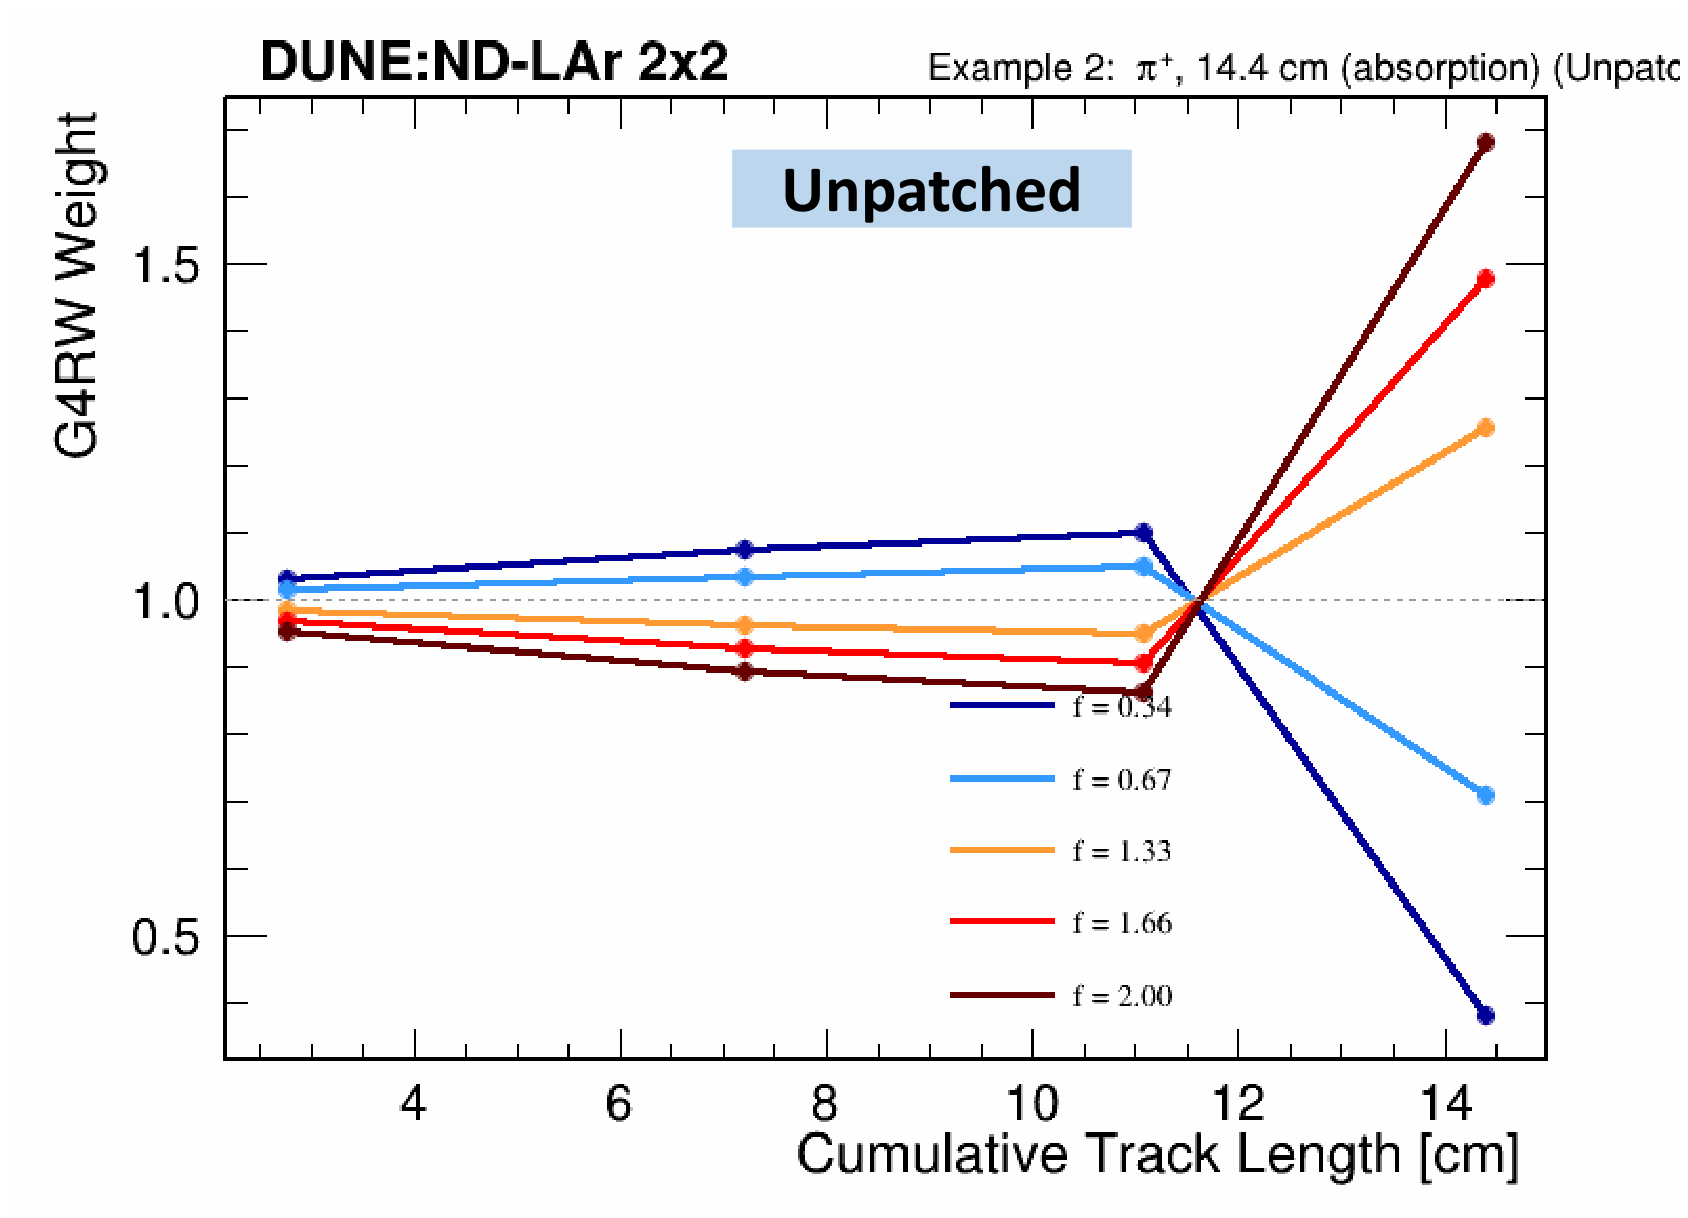
\includegraphics[width=0.48\textwidth]{fig08a_ex2_unpatched}\hfill
    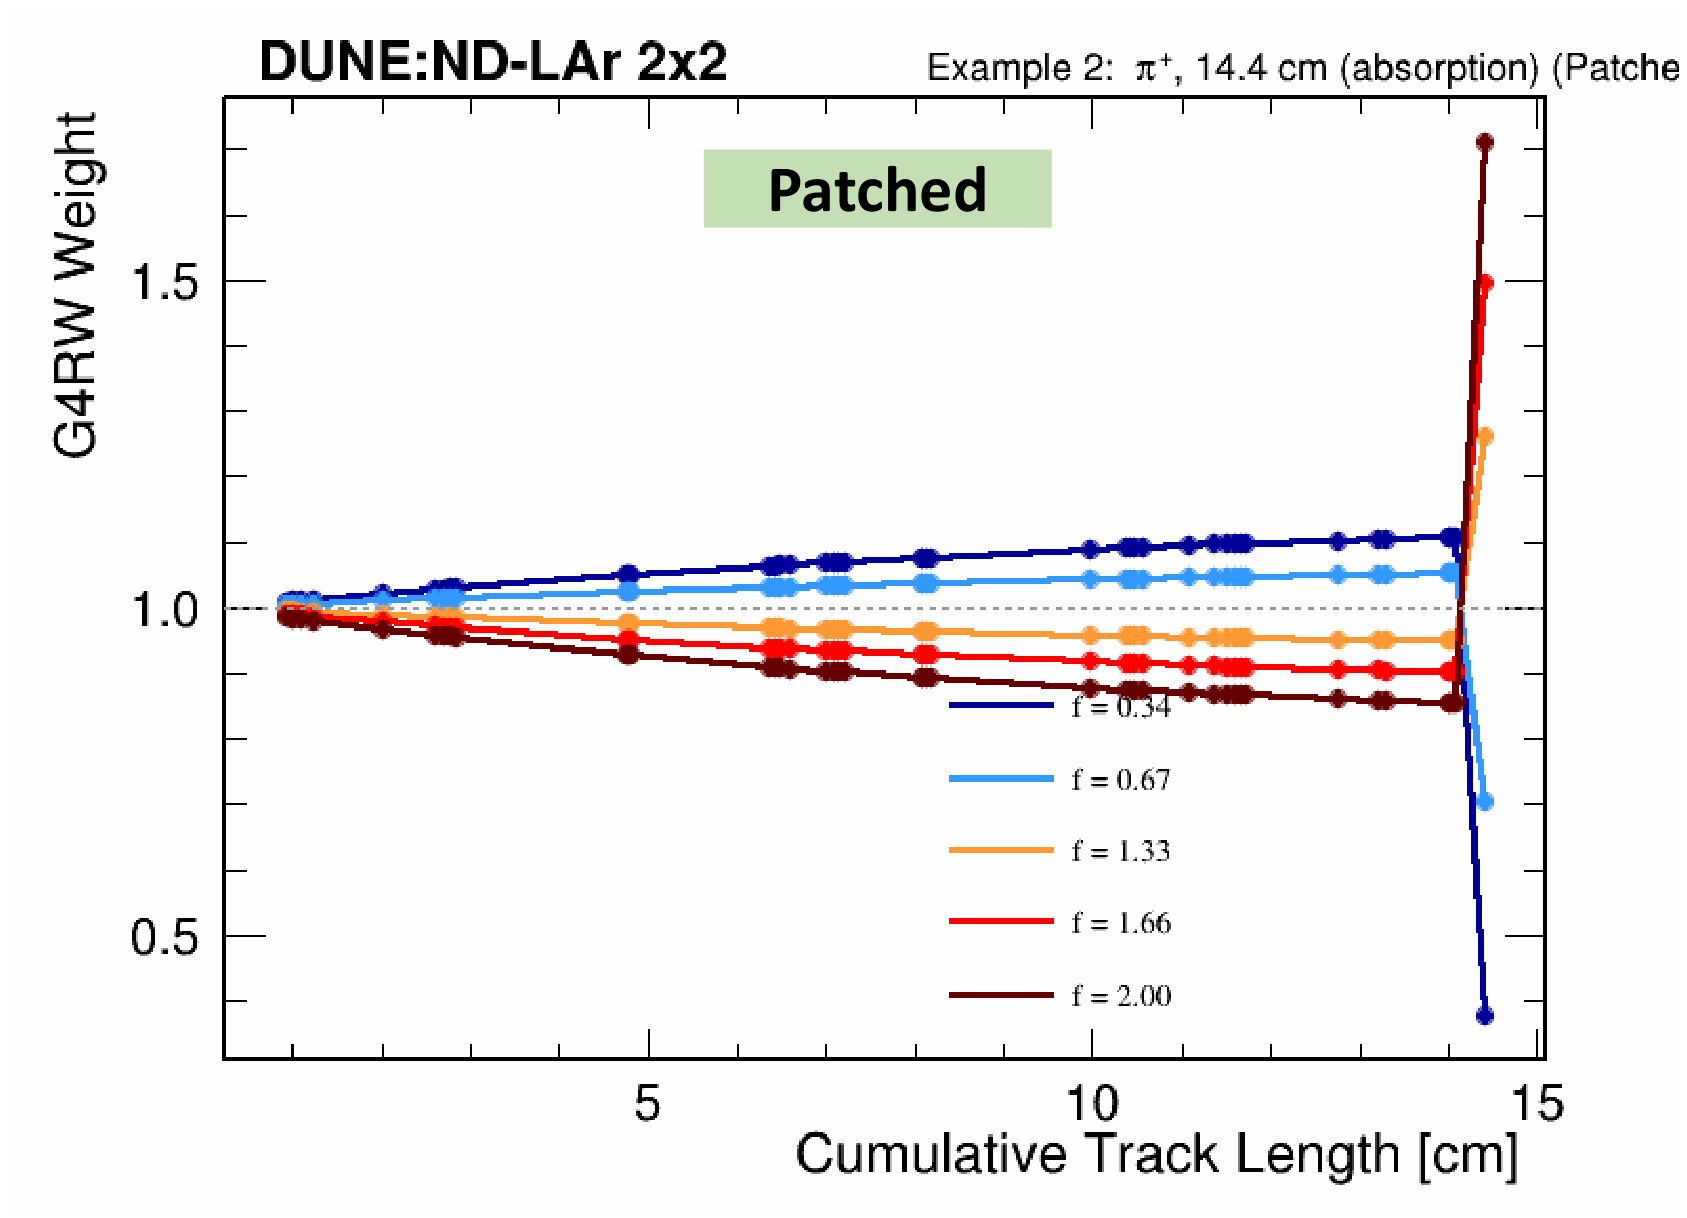
\includegraphics[width=0.48\textwidth]{fig08b_ex2_patched}
    \caption{Running weight against cumulative track length for
    Example 2, unpatched (left, four steps) and patched (right, 45 steps). The
    momentum falls by about $53\%$ along this track, and the patched curve
    follows the changing cross section step by step where the unpatched curve
    cannot.}
    \label{fig:example2_running}
\end{figure}
\fi

\subsection{\label{subsec:weight_dists}Weight Distributions}

Although we the SI systematic uncertainty is already implemented for  $\pi^+$, $\pi^-$, protons, and neutrons, we illustrate the results with detailed $\pi^+$ and proton examples.

Figure~\ref{fig:weight_dists} shows the weight distributions for truth
$\pi^{+}$ and truth protons from matched interactions (from CAFs), one curve per
scale factor. Taking $f = 1.33$ as representative, two features stand out
in both species: a distinct two-peak accumulation near $w = 1.00$ and
$w = 1.33$, and a tail of weights extending down towards zero.

% SOURCE: slides 8 and 32, "Truth PiPlus/Proton Weight Distribution: Patched Sample, All Scale Factors"
\begin{figure}[htb!]
    \centering
    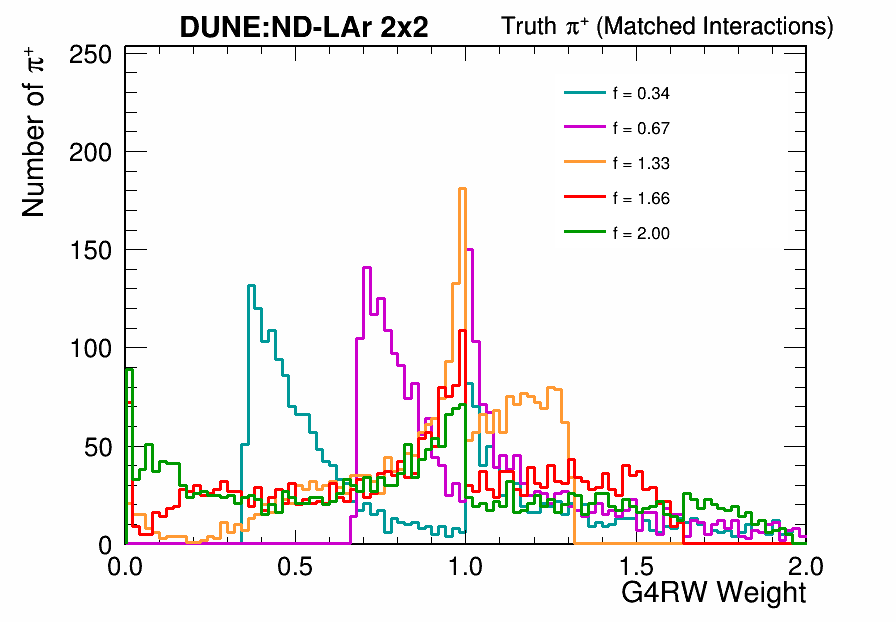
\includegraphics[width=0.48\textwidth]{fig09_piplus_weights}\hfill
    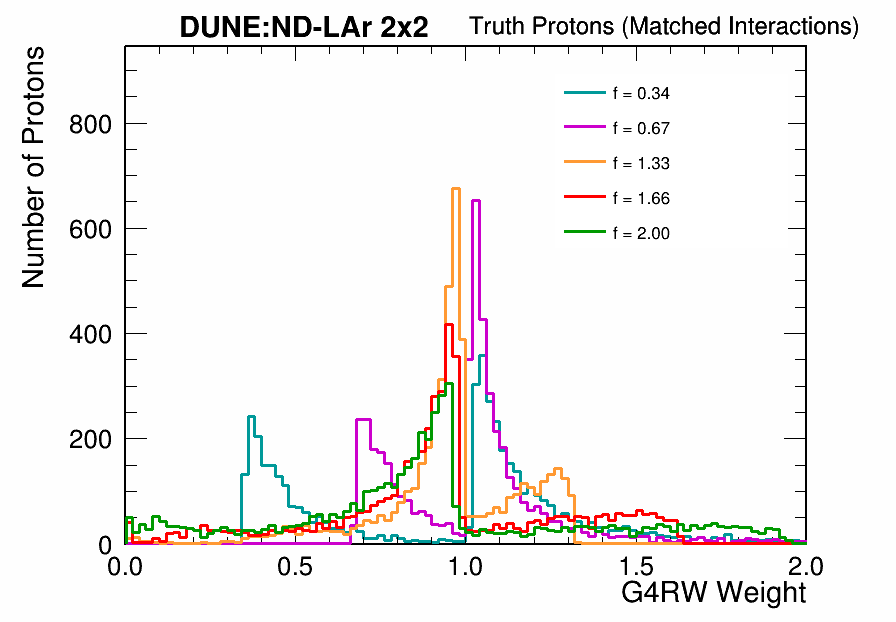
\includegraphics[width=0.48\textwidth]{fig10_proton_weights}
    \caption{G4RW weight distribution from matched interactions in the
    patched sample, one curve per cross-section scale factor, for truth
    $\pi^{+}$ (left) and truth protons (right). All five curves share the
    same general structure: a population accumulating near $w = 1.00$, a
    second near $w = f$, and a tail extending down towards zero.}
    \label{fig:weight_dists}
\end{figure}

Plotting the weight against track length separates the two populations
cleanly and explains both features directly. Figure~\ref{fig:track_length_2d}
shows the two-dimensional $\pi^{+}$ and proton distributions at
$f = 1.33$.

% SOURCE: slides 11 and 13, "Weight distribution as a function of Track Length for PiPlus/Protons"
\begin{figure}[htb!]
    \centering
    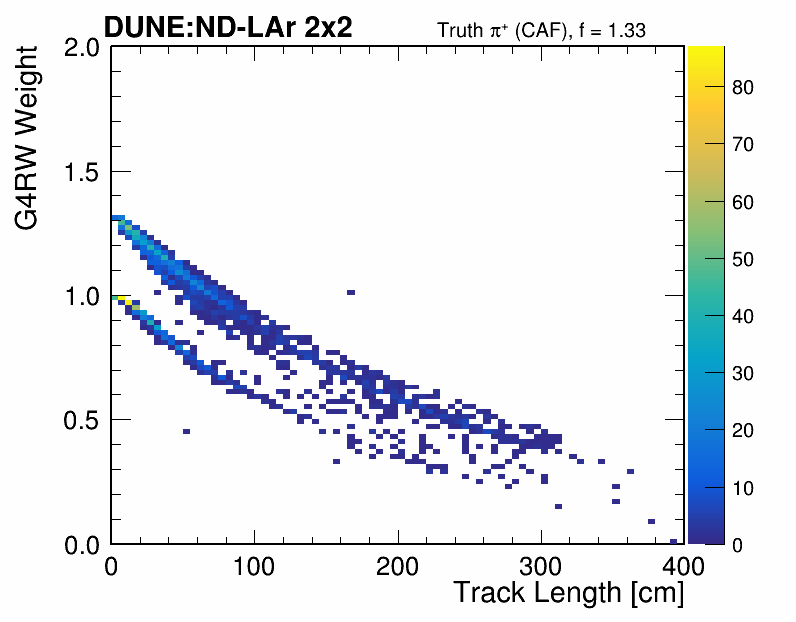
\includegraphics[width=0.48\textwidth]{fig11_piplus_2d}\hfill
    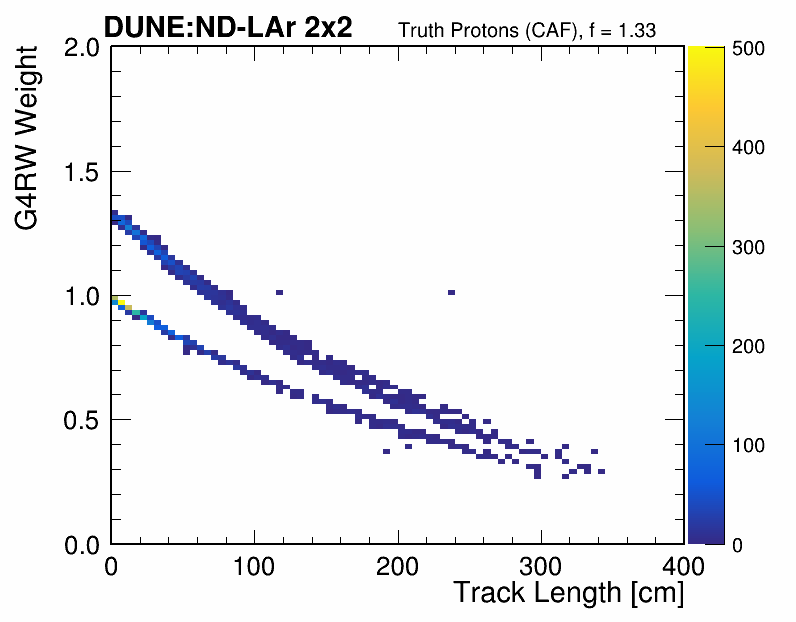
\includegraphics[width=0.48\textwidth]{fig12_proton_2d}
    \caption{Cumulative G4RW weight against truth track length at
    $f = 1.33$, for truth $\pi^{+}$ (left) and truth protons (right).
    Two bands are visible in both particle cases, converging near $w = 1.00$ and $w = 1.33$
    at short track length and falling together as the track lengthens. The
    lowest weights come from the longest tracks, which are predominantly
    those leaving the fiducial volume. The scattered entries sitting
    at $w = 1.00$ away from either band are hadrons with momentum above the
    upper edge of the fracs file.}
    \label{fig:track_length_2d}
\end{figure}

The two bands are the two terms of Eq.~\ref{eq:wtotal}. A track whose last
recorded point is tagged as a hadronic inelastic interaction receives both $W_S$
and $W_I$, and lands on the upper band, which starts near $w = f$ at zero length.
A track whose last point is tagged as anything else receives only $W_S$, and
lands on the lower band, which starts at $w = 1.00$. Both bands then fall with
track length as the survival term accumulates.

This can be tested directly by splitting on the \gfour{} process and subprocess
code recorded at each track's last point. Table~\ref{tab:last_point} gives the
composition and Figures~\ref{fig:piplus_split} and \ref{fig:proton_split} show
the resulting split.

% SOURCE: slides 12 and 14 (process fractions, merged)
\begin{table}[htb!]
\centering
\caption{Composition of the \gfour{} process/subprocess code at the
last recorded trajectory point, for truth $\pi^{+}$ and truth protons. Only the
hadron-inelastic category receives the interaction term of Eq.~\ref{eq:wi}.
Pions have a decay component that protons do not.}
\label{tab:last_point}
\setlength{\tabcolsep}{18pt}
\begin{tabular}{clcc}
\hline\hline
Geant4 Code (\texttt{proc}/\texttt{subproc}) & Meaning & $\pi^{+}$ & proton \\
\hline
4/121 & hadron inelastic              & 70.3\% & 41.8\% \\
2/22  & electromagnetic/scintillation & 26.4\% & 58.2\% \\
6/201 & decay                         &  3.3\% & --- \\
\hline\hline
\end{tabular}
\end{table}

% SOURCE: slide 12, "Examining via Geant4 Process/Subprocess Tags" (pion)
\begin{figure}[htb!]
    \centering
    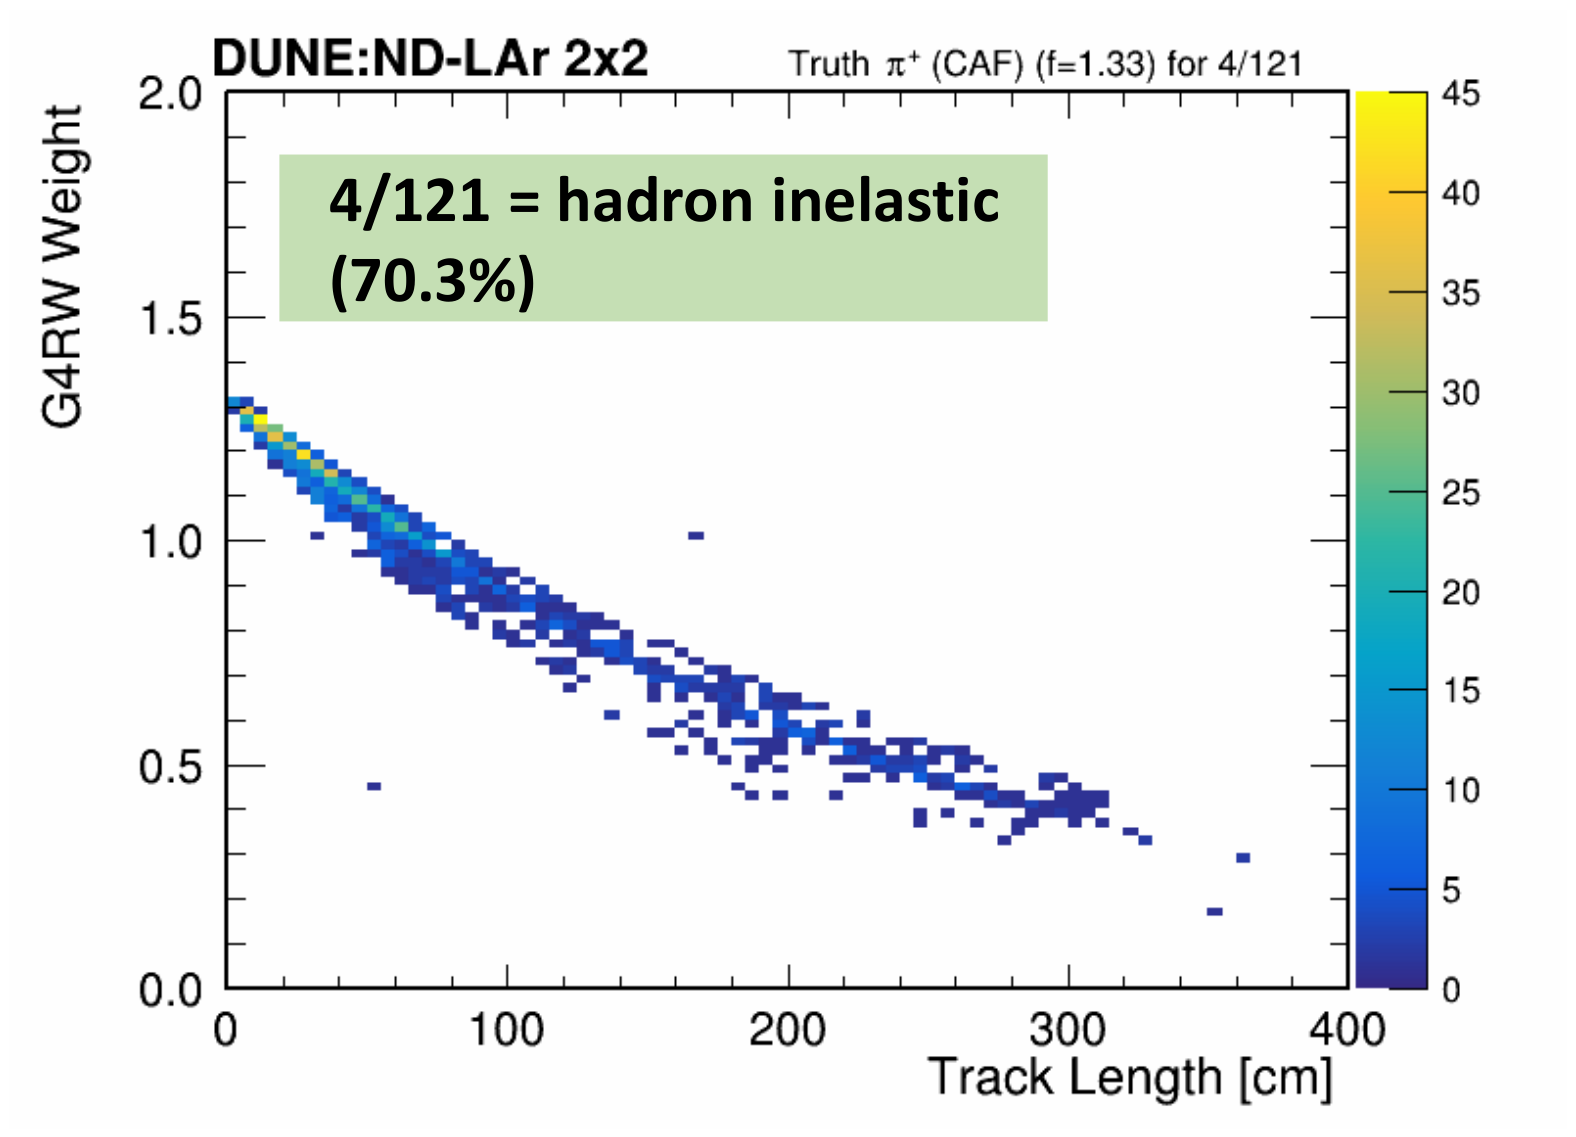
\includegraphics[width=0.50\textwidth]{fig13a_pi_inelastic}\\[6pt]
    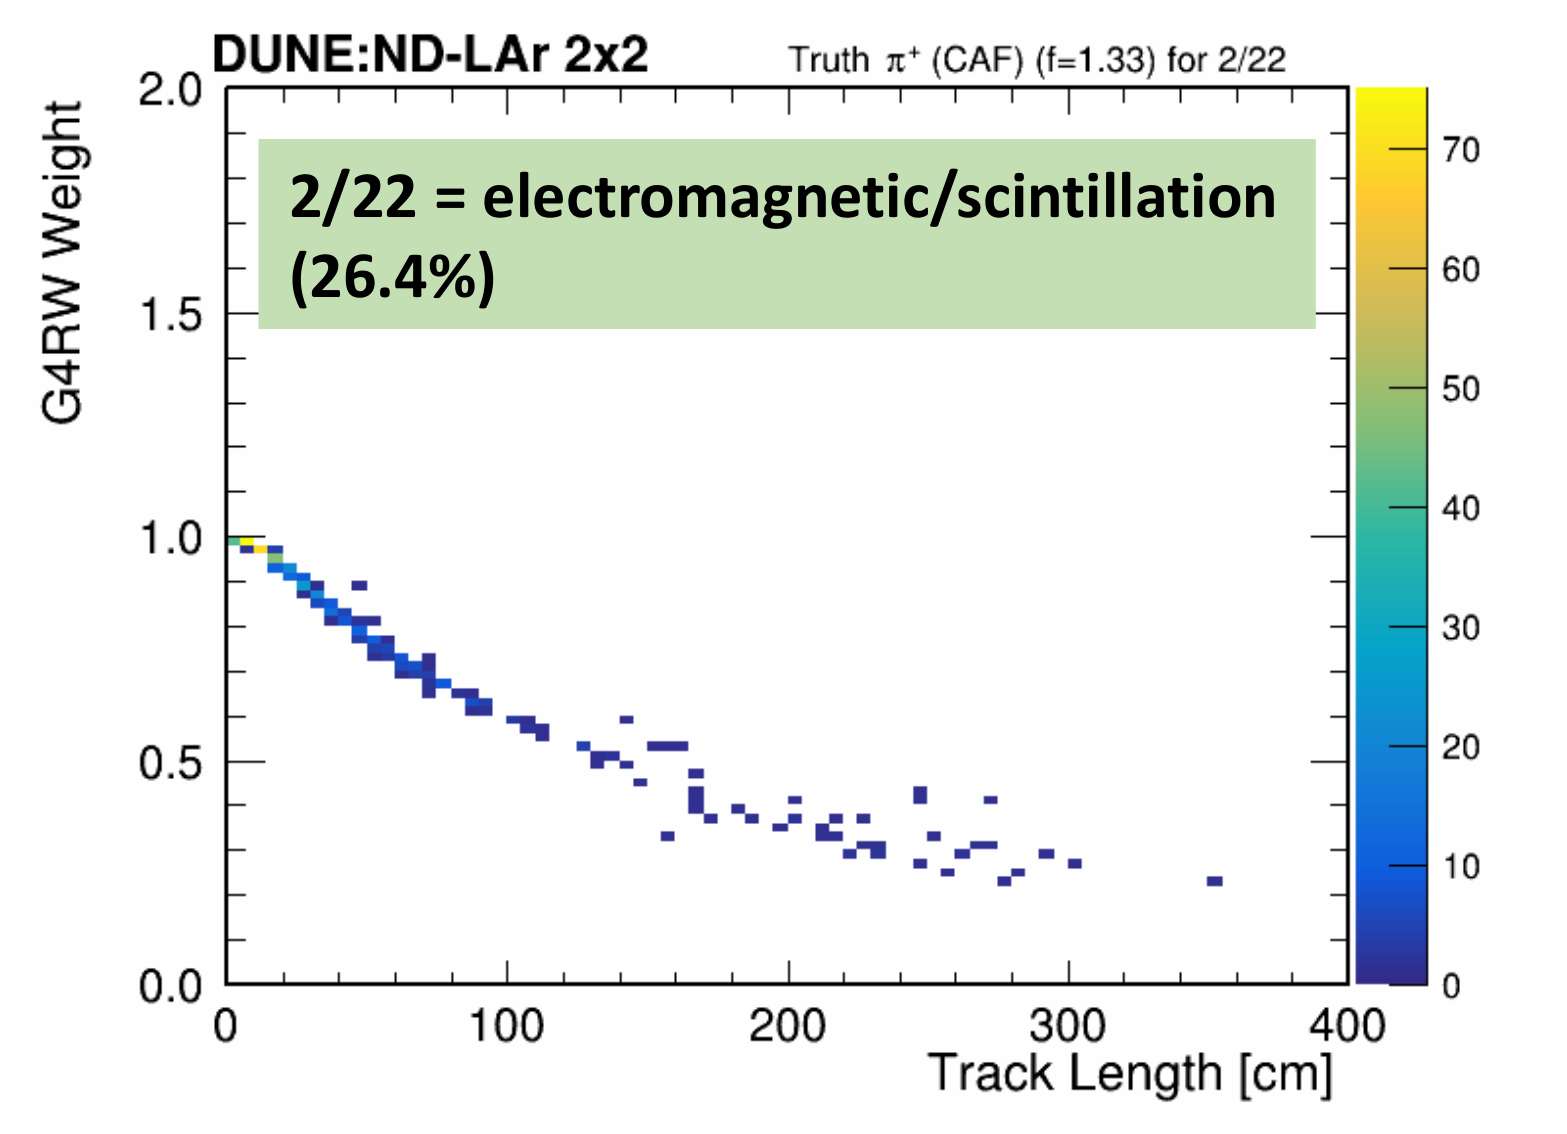
\includegraphics[width=0.50\textwidth]{fig13b_pi_em}\hfill
    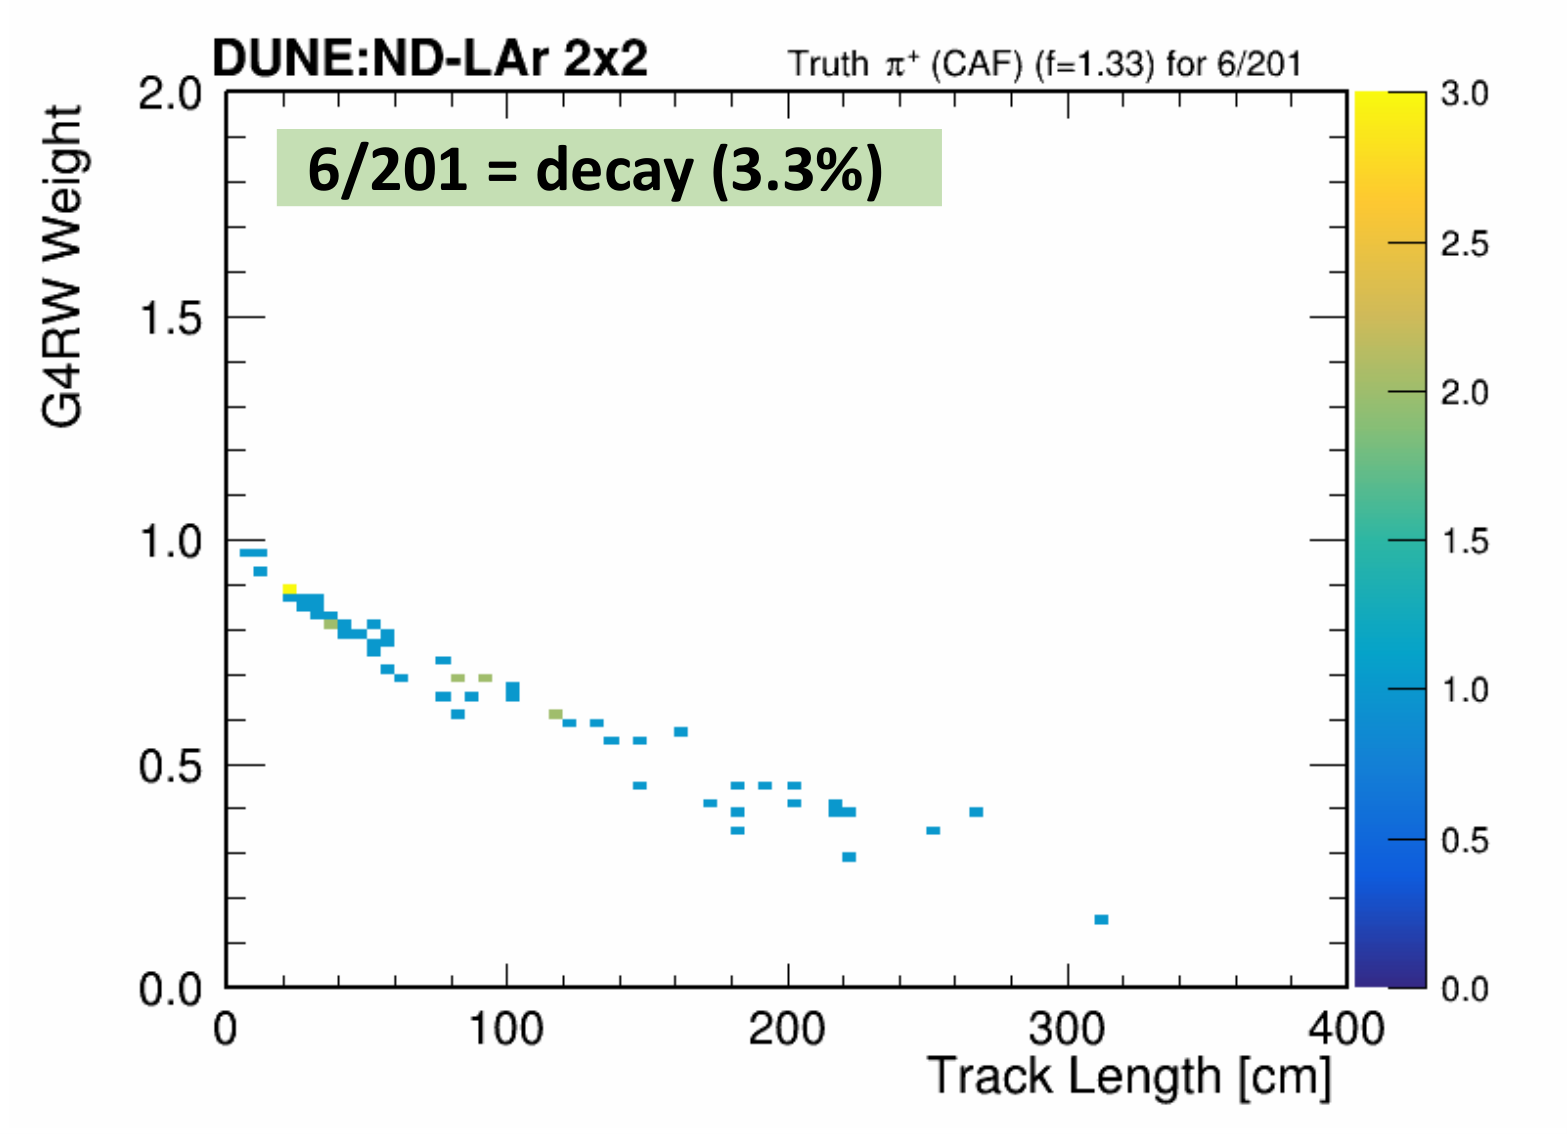
\includegraphics[width=0.50\textwidth]{fig13c_pi_decay}
    \caption{Weight against track length for truth $\pi^{+}$ at
    $f = 1.33$, split by the \gfour{} process/subprocess code at the last
    recorded point: hadron inelastic (4/121, top), electromagnetic/scintillation
    (2/22, bottom left), and decay (6/201, bottom right). Only the first begins
    at $w = f$; the other two begin at $w = 1.00$, confirming that the upper
    band is exactly the population receiving the interaction term.}
    \label{fig:piplus_split}
\end{figure}

% SOURCE: slide 14, "Examining via Geant4 Process/Subprocess Tags" (proton)
\begin{figure}[htb!]
    \centering
    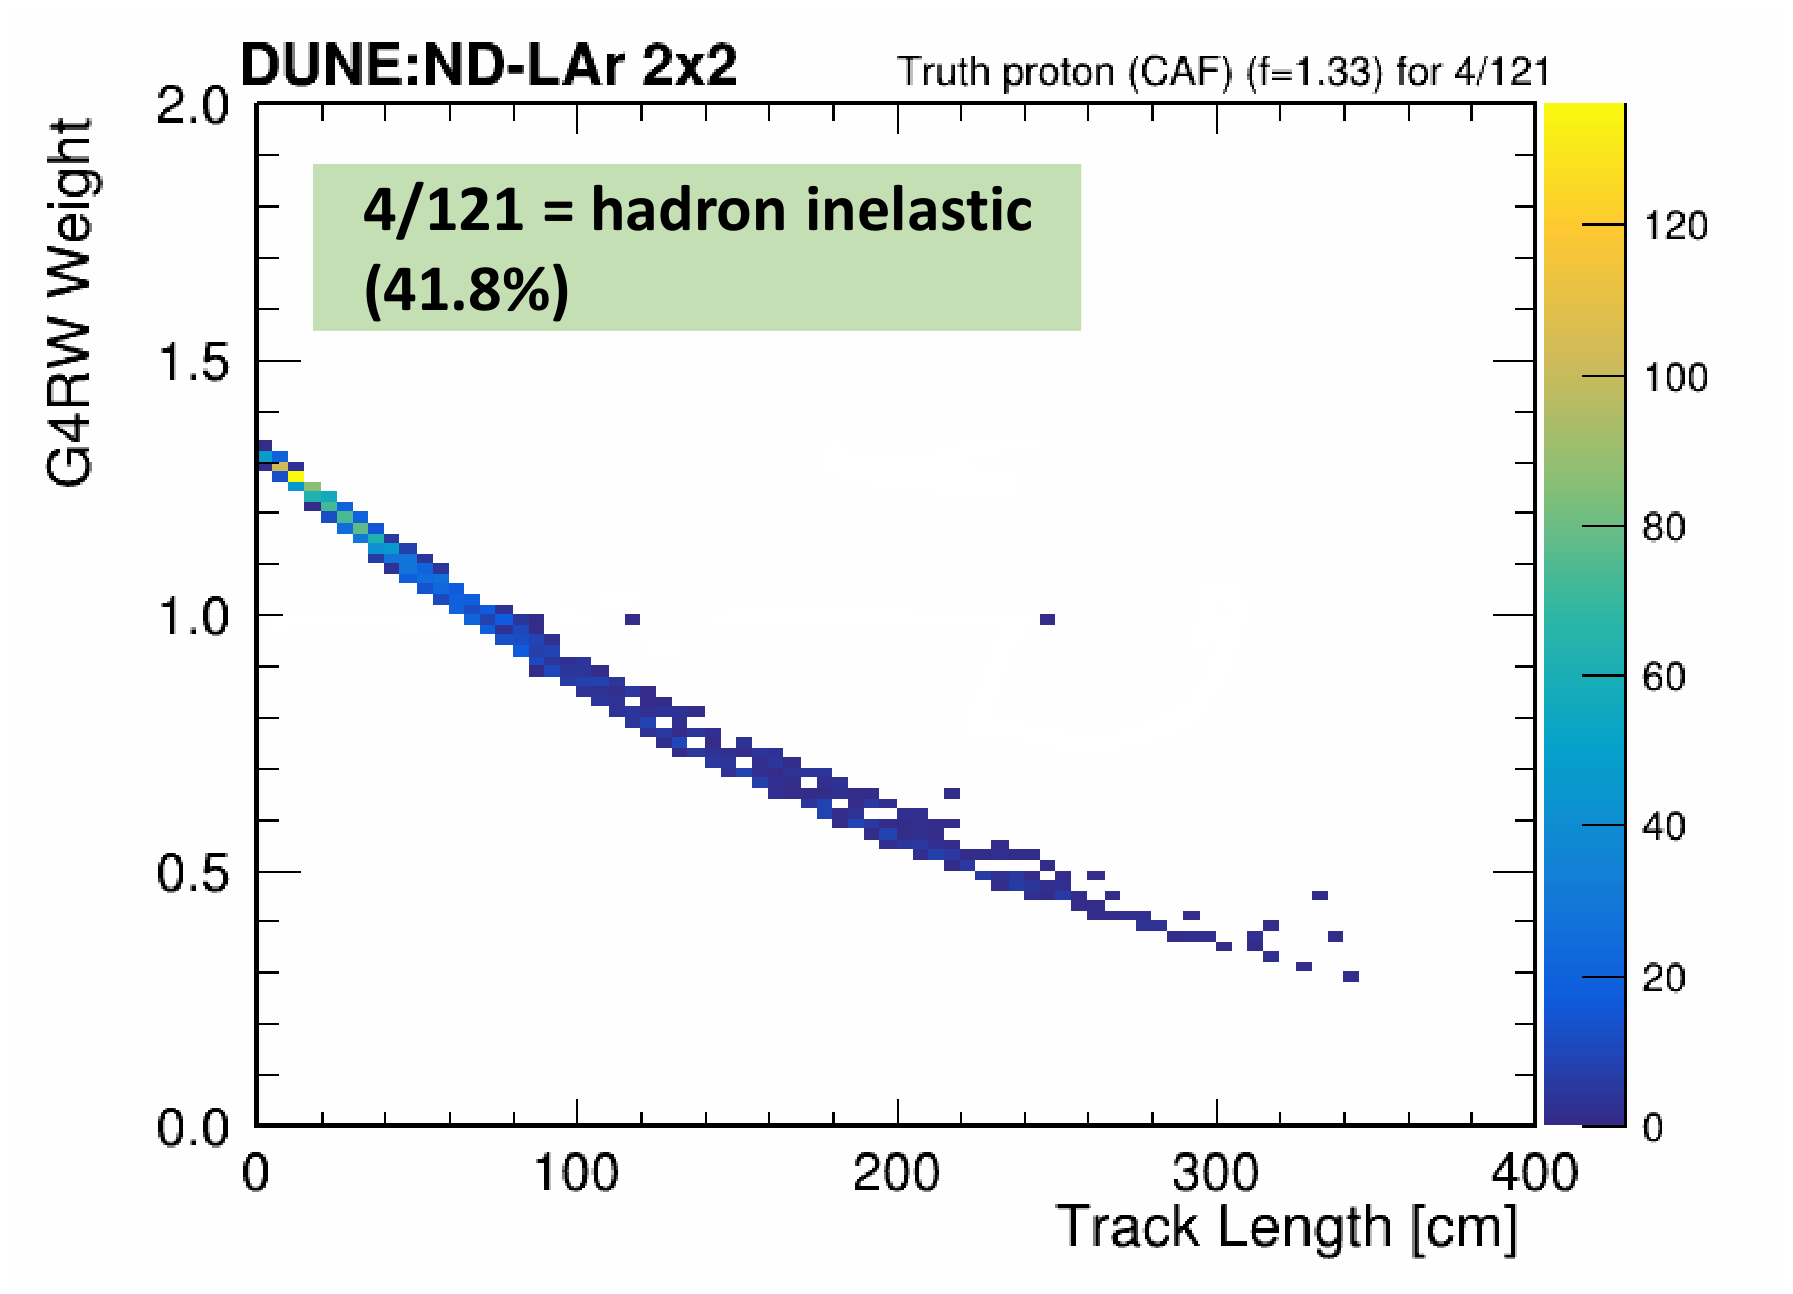
\includegraphics[width=0.48\textwidth]{fig14a_p_inelastic}\hfill
    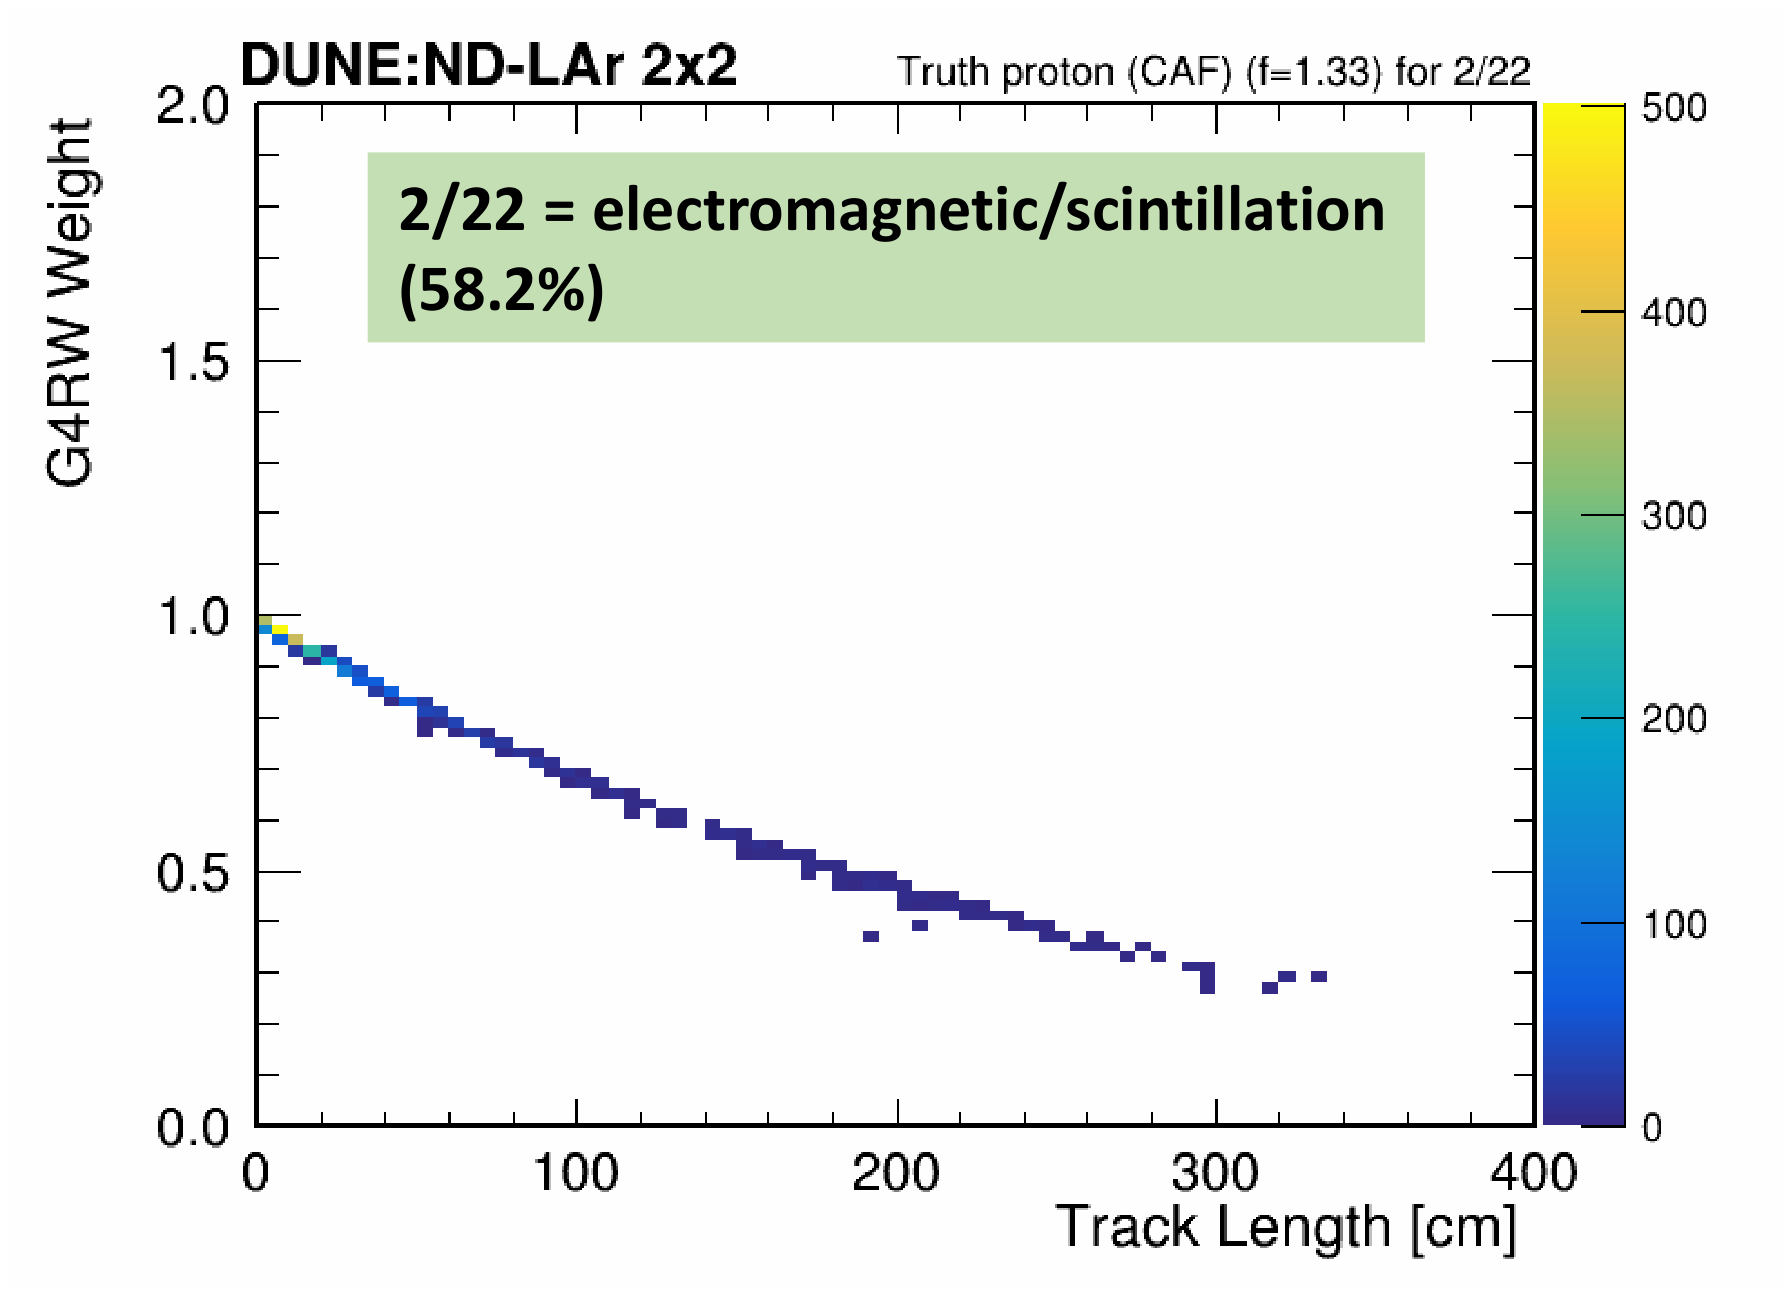
\includegraphics[width=0.48\textwidth]{fig14b_p_em}
    \caption{Weight against track length for truth protons at
    $f = 1.33$, split by the \gfour{} process/subprocess code at the last
    recorded point. Protons divide between hadron inelastic (4/121) and
    electromagnetic/scintillation (2/22) only.}
    \label{fig:proton_split}
\end{figure}

\iffalse
% SOURCE: slide 30, "Understanding the Two Trends: Geant4 Process/Subprocess Codes"
\begin{figure}[H]
    \centering
    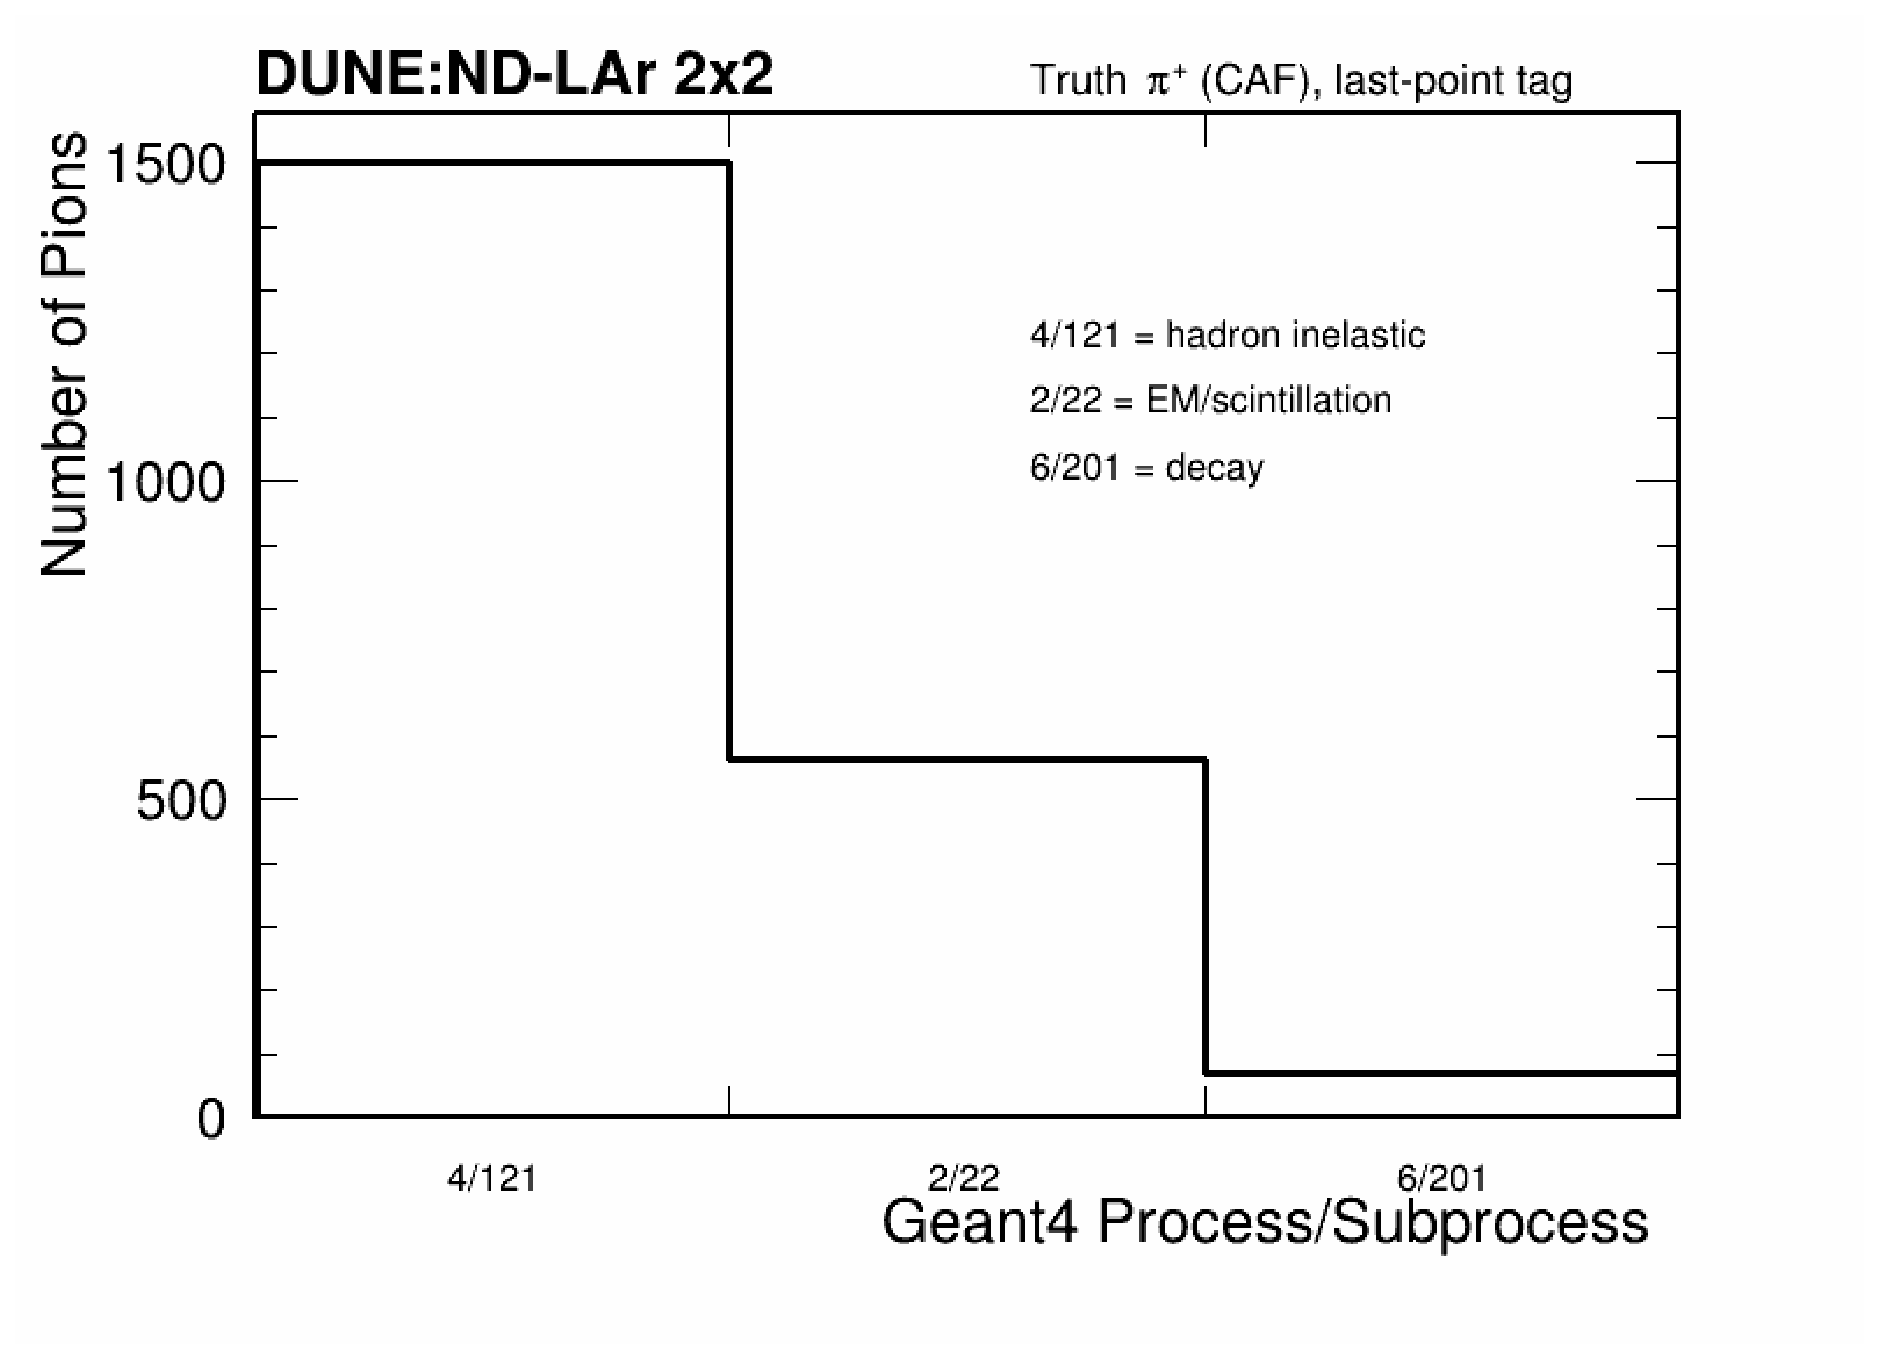
\includegraphics[width=0.62\textwidth]{fig15_last_point_bar}
    \caption{Number of truth $\pi^{+}$ by \gfour{}
    process/subprocess code at the last recorded trajectory point, giving the
    composition quoted in Table~\ref{tab:last_point}.}
    \label{fig:last_point_bar}
\end{figure}
\fi

The difference between the two species in Table~\ref{tab:last_point} is worth
noting. Protons end in a hadronic inelastic interaction only $41.8\%$ of the
time against $70.3\%$ for pions, with the remainder stopping by ionisation.
Fewer proton tracks therefore receive an interaction term, which is why the
$w = 1.00$ peak is relatively more prominent for protons than for pions in
Figure~\ref{fig:weight_dists}.

Some scattered entries at $w = 1.00$ in Figure~\ref{fig:track_length_2d} are those hadrons whose momentum exceeds the upper edge of the
fracs file ($ |p| > $9001~MeV/$c$; Section~\ref{subsec:fracs}), where the channel decomposition is undefined and no scaling is
applied. 


% ===========================================================================
\section{\label{sec:si_weight_parameterization}SI Weight Parameterization vs.\ True Track Length}
% ===========================================================================

The weight interface described so far is a per-hadron lookup: each weight is
retrieved using the key (\texttt{cafFileIdx}, \texttt{nu\_id},
\texttt{G4ID}), and exists only for hadrons that were generated and produced a
matching entry in the weight file (Section~\ref{subsec:matching}).

This framework is complete, and its use is demonstrated in Section~\ref{sec:analysis_examples} (Figures~\ref{fig:proton_si_band}, \ref{fig:proton_truth_reco},
and~\ref{fig:multiplicity}). We extended it with a continuous parameterization
of the weight as a function of the true track length $L$, a polynomial
$w(L) = \sum_{k=0}^{n} c_k\, L^k$ fit to the scatter of per-hadron weights
already produced by the framework. The parameterization gives the weight at
any point in true or reconstructed phase space; in particular, for a hadron
that leaves the fiducial volume, it can be evaluated at the true length
accumulated up to the point where the hadron exits the detector.

The scatter separates into two populations with distinct weight-length
trends, identified using the Geant4 process/subprocess tag at each hadron's
last recorded point: hadrons whose last point is tagged hadronic-inelastic
($4/121$), versus hadrons whose last point is tagged something other than
$4/121$. We examine this separately for protons and $\pi^+$, using the same
$[5,290]$~cm fit range for both populations of each species.

We tested polynomial fits of order 3 through 7 for both populations of each
species. Figures~\ref{fig:proton_2d_fit} and~\ref{fig:piPlus_2d_fit}, together
with Tables~\ref{tab:proton_2d_fit_L200} and~\ref{tab:piPlus_2d_fit_L200},
show the fitted weight at $L=200$~cm for each order; across all four cases
(proton and $\pi^+$, each tagged $4/121$ or tagged other than $4/121$), pol3
is the simplest solution, with a minimal fit uncertainty when compared  to other polynomial fits tested.

% SOURCE: slides 21-22, "Weights as a Function of Track Length for
% Hadronic/No-Hadronic Interaction for Protons"
\begin{figure}[htb!]
    \centering
    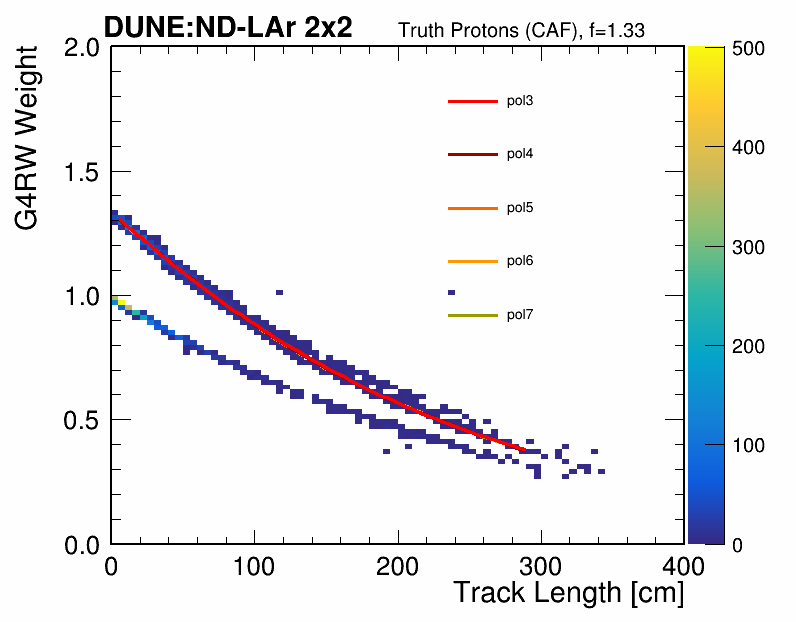
\includegraphics[width=0.50\textwidth]{fig12_proton_2d_fit_upper}\hfill
    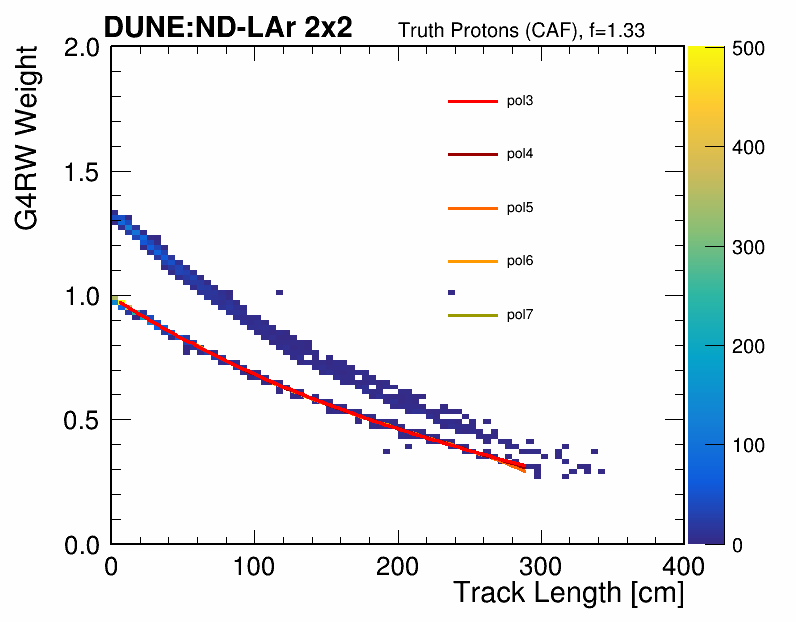
\includegraphics[width=0.50\textwidth]{fig12_proton_2d_fit_lower}
    \caption{Preliminary polynomial fits (order 3--7) to G4RW weight
    ($f=1.33$) vs.\ true track length for truth protons, separated
    by the Geant4 process/subprocess tag at each track's last recorded
    trajectory point: last point tagged hadronic-inelastic, $4/121$ (left),
    and last point tagged something other than $4/121$ (right).}
    \label{fig:proton_2d_fit}
\end{figure}

\begin{table}[htb!]
\centering
\caption{Fitted G4RW weight at $L=200$~cm, by polynomial order, for protons
whose last trajectory point is tagged hadronic-inelastic ($4/121$) versus
tagged something other than $4/121$.}
\label{tab:proton_2d_fit_L200}
\setlength{\tabcolsep}{12pt}
\begin{tabular}{lcc}
\hline\hline
Order & $w(L=200\,\text{cm})$, $4/121$ & $w(L=200\,\text{cm})$, other than $4/121$ \\
\hline
pol3 & $0.5663 \pm 0.0012$ & $0.4631 \pm 0.0009$ \\
pol4 & $0.5660 \pm 0.0012$ & $0.4638 \pm 0.0010$ \\
pol5 & $0.5661 \pm 0.0016$ & $0.4636 \pm 0.0010$ \\
pol6 & $0.5670 \pm 0.0019$ & $0.4644 \pm 0.0012$ \\
pol7 & $0.5668 \pm 0.0023$ & $0.4644 \pm 0.0012$ \\
\hline\hline
\end{tabular}
\end{table}

A $\pi^+$ whose last point is \emph{not} tagged hadronic-inelastic can reach
that state via two distinct processes: electromagnetic/scintillation
($2/22$) or decay ($6/201$). The lower-population curve in
Figure~\ref{fig:piPlus_2d_fit} is drawn only up to $L=240$~cm: beyond that
point per-length-bin statistics decrease sharply (several bins with only
2--5 tracks), and the higher-order fits (pol6, pol7) become visibly unstable
there. The fit itself still uses the full $[5,290]$~cm range; only the drawn
range is truncated.

% SOURCE: slides (piPlus), "Weights as a Function of Track Length for
% Hadronic/No-Hadronic Interaction for PiPlus"
\begin{figure}[htb!]
    \centering
    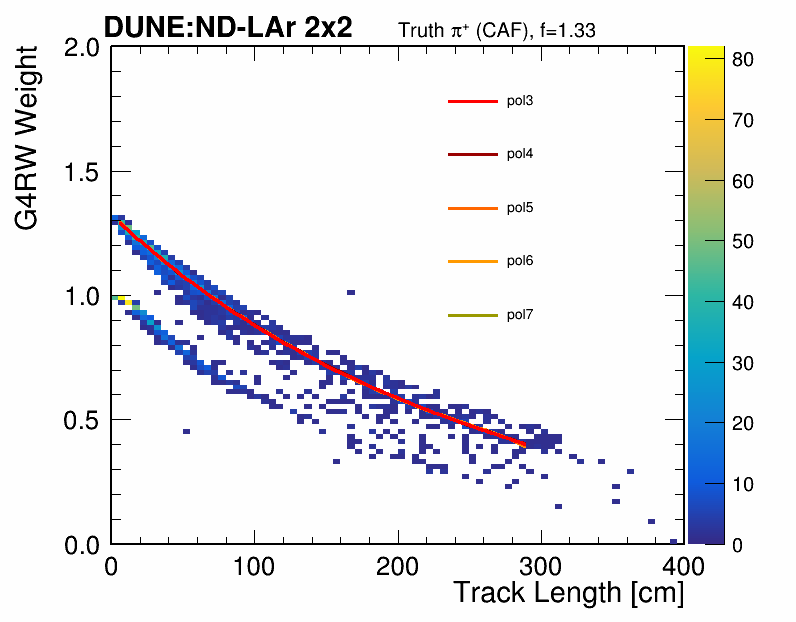
\includegraphics[width=0.50\textwidth]{fig12_piPlus_2d_fit_upper}\hfill
    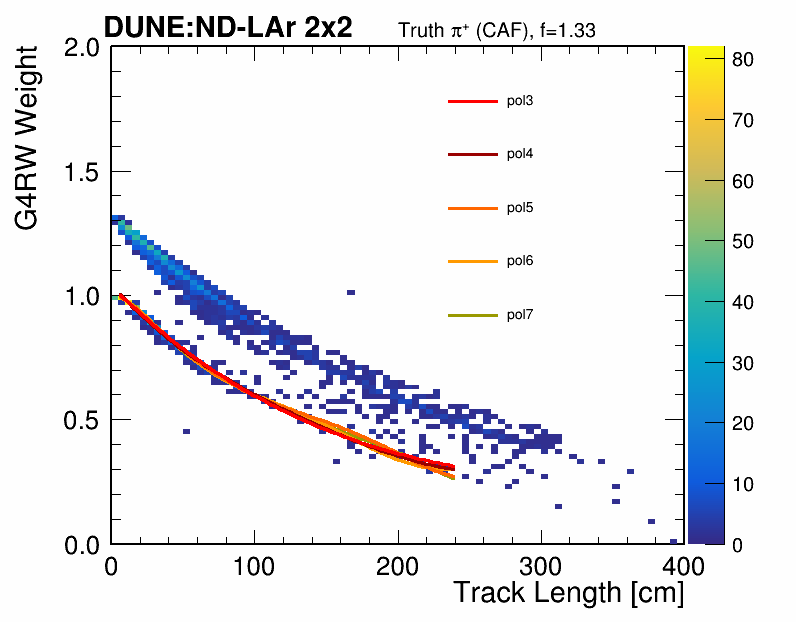
\includegraphics[width=0.50\textwidth]{fig12_piPlus_2d_fit_lower}
    \caption{Preliminary polynomial fits (order 3--7) to G4RW weight
    ($f=1.33$) vs.\ true track length for truth $\pi^+$, separated
    by the Geant4 process/subprocess tag at each track's last recorded
    trajectory point: last point tagged hadronic-inelastic, $4/121$ (left),
    and last point tagged something other than $4/121$ (right, drawn over
    $[5,240]$~cm, see text).}
    \label{fig:piPlus_2d_fit}
\end{figure}

\begin{table}[htb!]
\centering
\caption{Fitted G4RW weight at $L=200$~cm, by polynomial order, for $\pi^+$
whose last trajectory point is tagged hadronic-inelastic ($4/121$) versus
tagged something other than $4/121$.}
\label{tab:piPlus_2d_fit_L200}
\setlength{\tabcolsep}{12pt}
\begin{tabular}{lcc}
\hline\hline
Order & $w(L=200\,\text{cm})$, $4/121$ & $w(L=200\,\text{cm})$, other than $4/121$ \\
\hline
pol3 & $0.5861 \pm 0.0017$ & $0.3645 \pm 0.0033$ \\
pol4 & $0.5862 \pm 0.0017$ & $0.3539 \pm 0.0038$ \\
pol5 & $0.5846 \pm 0.0021$ & $0.3651 \pm 0.0039$ \\
pol6 & $0.5840 \pm 0.0023$ & $0.3387 \pm 0.0049$ \\
pol7 & $0.5841 \pm 0.0026$ & $0.3678 \pm 0.0063$ \\
\hline\hline
\end{tabular}
\end{table}

Given this stability, the pol3 fit is adopted as the parameterization,
\begin{equation}
\label{eq:pol3_form}
w(L) = c_0 + c_1 L + c_2 L^2 + c_3 L^3,
\end{equation}
with $L$ in cm. Tables~\ref{tab:pol3_coefficients_proton} and
\ref{tab:pol3_coefficients_piPlus} list the fitted coefficients, with
propagated errors, for protons and $\pi^+$ respectively.

\begin{table}[htb!]
\centering
\small
\caption{Fitted pol3 coefficients (Eq.~\ref{eq:pol3_form}) for protons, with
propagated errors.}
\label{tab:pol3_coefficients_proton}
\setlength{\tabcolsep}{6pt}
\begin{tabular}{lcccc}
\hline\hline
Population & $c_0$ & $c_1$ & $c_2$ & $c_3$ \\
\hline
$4/121$
 & $1.3371(\pm0.0013)$
 & $-5.2975(\pm0.0541)\times10^{-3}$
 & $7.9967(\pm0.4791)\times10^{-6}$
 & $-3.8995(\pm1.1614)\times10^{-9}$ \\
other than $4/121$
 & $0.9941(\pm0.0006)$
 & $-3.6969(\pm0.0307)\times10^{-3}$
 & $6.4614(\pm0.3297)\times10^{-6}$
 & $-6.2622(\pm0.9220)\times10^{-9}$ \\
\hline\hline
\end{tabular}
\end{table}

\begin{table}[htb!]
\centering
\small
\caption{Fitted pol3 coefficients (Eq.~\ref{eq:pol3_form}) for $\pi^+$, with
propagated errors.}
\label{tab:pol3_coefficients_piPlus}
\setlength{\tabcolsep}{6pt}
\begin{tabular}{lcccc}
\hline\hline
Population & $c_0$ & $c_1$ & $c_2$ & $c_3$ \\
\hline
$4/121$
 & $1.3241(\pm0.0022)$
 & $-5.4381(\pm0.0851)\times10^{-3}$
 & $1.0925(\pm0.0762)\times10^{-5}$
 & $-1.0915(\pm0.1904)\times10^{-8}$ \\
other than $4/121$
 & $1.0356(\pm0.0017)$
 & $-5.6875(\pm0.0922)\times10^{-3}$
 & $1.4203(\pm0.1049)\times10^{-5}$
 & $-1.2708(\pm0.2847)\times10^{-8}$ \\
\hline\hline
\end{tabular}
\end{table}


% ===========================================================================
\section{\label{sec:propagation}Propagation to Truth and Reconstructed Observables}
% ===========================================================================

\subsection{\label{subsec:matching}Matching Weights to Reconstructed and Truth-Level Particles}

The SI weights are computed on MiniRun5 EDepSim files, but the observables,
both reconstructed and truth-level, are read from MiniRun6.5 CAF files. Three
files must therefore be linked: the EDepSim file, the weight file, and the CAF
file.

Files correspond one to one by index. Within a file, interactions are matched by
a unique identifier built from the EDepSim run and event numbers,
\begin{equation}
\label{eq:vertex_id}
\texttt{event\_id} = \texttt{RunId} \times 10^{6} + \texttt{EventId},
\end{equation}
where \texttt{RunId} encodes which of the ten GENIE sub-files inside a merged
EDepSim file the interaction came from and \texttt{EventId} counts interactions
within that sub-file. This identifier survives the full chain
(GENIE $\rightarrow$ EDepSim $\rightarrow$ \texttt{larnd-sim} $\rightarrow$ FLOW $\rightarrow$ SPINE $\rightarrow$ CAF)
and appears in the CAF as \texttt{nu.id}. Individual particles are matched by
the \gfour{} track identifier, stored as \texttt{prim.G4ID} in the CAF.

The three-way key is summarised in Table~\ref{tab:matching_key}. Because the key
is built entirely from truth-level identifiers (\texttt{G4ID}, \texttt{nu.id}),
it resolves identically regardless of whether the resulting weight is applied to
a particle's true or reconstructed kinematics; Section~\ref{subsec:proton_results}
uses this to apply the same SI weight map to both the reconstructed and
truth-level track length of a common set of backtracked proton candidates. A
worked implementation of both the reconstructed and truth-level fills is
available in the multiplicity analysis code~\cite{proton_plots_repo}, commit
\texttt{ab109f6} (reconstructed fill: lines 3300--3324; truth fill: lines
3328--3347).

\begin{table}[H]
\centering
\caption{The three-way lookup key linking CAF, weight, and EDepSim files.}
\label{tab:matching_key}
\setlength{\tabcolsep}{18pt}
\begin{tabular}{lccc}
\hline\hline
File & File index & Interaction ID & Particle ID \\
\hline
CAF     & loop index $f$     & \texttt{nu.id}   & \texttt{prim.G4ID} \\
Weights & \texttt{file\_idx} & \texttt{event\_id} & \texttt{track\_id} \\
EDepSim & filename index     & $\texttt{RunId}\times10^{6} + \texttt{EventId}$ & \texttt{TrackId} \\
\hline\hline
\end{tabular}
\end{table}

A particle with no entry in the weight map receives $w = 1.0$ and contributes no shift. 
% This covers particles that underwent no inelastic interaction, and rock
% hadrons, which are absent from the ANL samples by construction.

\subsection{\label{subsec:application}Building the Systematic Band}

Weights are applied when filling histograms. Each entry falls in one bin, and
for each observable this gives a nominal and a shifted histogram,
\begin{equation}
\label{eq:hist_pair}
h^{\text{nom}}_i = \sum_{\text{entries in bin } i} 1,
\qquad
h^{\text{wt}}_i = \sum_{\text{entries in bin } i} w .
\end{equation}


Since the current production supplies one weight per particle per scale factor,
the shift in bin $i$ is
\begin{equation}
\label{eq:unisim_shift}
\delta_i = h^{\text{wt}}_i - h^{\text{nom}}_i ,
\end{equation}
and the uncertainty band in the figures is $\sigma_i = |\delta_i|$, using
only that bin's own shift. 

The band construction above depends only on each track's weight $w$, not on how it was obtained, so it applies equally whether $w$ is evaluated from the fitted parameterization of Section~\ref{sec:si_weight_parameterization} or a bare weight in the G4RW output ROOT files (Section~\ref{subsec:matching}).

% Old v2

% \subsection{\label{subsec:application}Building the Systematic Band}

% Weights are applied when filling histograms. Each entry falls in one bin, and
% for each observable this gives a nominal and a shifted histogram,
% \begin{equation}
% \label{eq:hist_pair}
% h^{\text{nom}}_i = \sum_{\text{entries in bin } i} 1,
% \qquad
% h^{\text{wt}}_i = \sum_{\text{entries in bin } i} w .
% \end{equation}

% % in direct analogy with the \texttt{nusystematics} treatment of interaction
% % uncertainties.

% Since the current production supplies one weight per particle per scale factor,
% the covariance is built with the unisim (single-universe) method. The shift in
% bin $i$ is
% \begin{equation}
% \label{eq:unisim_shift}
% \delta_i = h^{\text{wt}}_i - h^{\text{nom}}_i ,
% \end{equation}
% and, because all bins are shifted by the same single variation of the scale
% factor, the covariance between any two bins $i$ and $j$ is
% \begin{equation}
% \label{eq:unisim_cov}
% C_{ij} = \delta_i\,\delta_j .
% \end{equation}
% The uncertainty band in the figures is built from the diagonal elements of
% this matrix, $\sigma_i = \sqrt{C_{ii}} = |\delta_i|$.


% Old v1

% \subsection{\label{subsec:application}Building the Systematic Band}

% Weights are applied when filling histograms. The reconstructed values themselves
% are untouched; only the fill weight changes. For each observable this gives a
% nominal and a shifted histogram,
% \begin{equation}
% \label{eq:hist_pair}
% h^{\text{nom}}_i = \sum_{\text{entries in bin } i} 1,
% \qquad
% h^{\text{wt}}_i = \sum_{\text{entries in bin } i} w .
% \end{equation}

% % in direct analogy with the \texttt{nusystematics} treatment of interaction
% % uncertainties.

% Since the current production supplies one weight per particle per scale factor,
% the covariance is built with the unisim (single-universe) method. The shift in
% bin $i$ is
% \begin{equation}
% \label{eq:unisim_shift}
% \delta_i = h^{\text{wt}}_i - h^{\text{nom}}_i ,
% \end{equation}
% and the covariance matrix is the outer product of the shift vector with itself,
% \begin{equation}
% \label{eq:unisim_cov}
% C_{ij} = \delta_i\,\delta_j .
% \end{equation}
% The per-bin uncertainty is $\sigma_i = \sqrt{C_{ii}} = |\delta_i|$. This matrix
% is rank one by construction: it has a single non-zero eigenvalue and every bin
% is perfectly correlated or anti-correlated with every other through the one
% shift vector. 

% % That is the correct description when a single scale factor is
% % varied, but it cannot represent independent shape variation --- which is the
% % main reason for moving to multisim (Section~\ref{subsec:next_multisim}).

% ===========================================================================
\section{\label{sec:analysis_examples}Analysis Examples with Incorporated SI, GENIE, and Detector Systematics}
% ===========================================================================

In this section, we incorporate systematics uncertainties from SI, nusystematics, and detector response in two example analyses; in both, the SI weight is the bare weight from the G4RW output ROOT files (Section~\ref{subsec:matching}), not the fitted parameterization of Section~\ref{sec:si_weight_parameterization}.

\subsection{\label{subsec:proton_results}Example of SI Systematics in Reconstructed and Truth-Level Proton Track Length}

As we study charged hadron multiplicity, we need to understand the individual primary particle distribution. To that end we looked at the proton sample, and used it as a test bed for incorporating the SI systematic uncertainty, as well as all other systematic contributions as described in this section.

Figure~\ref{fig:proton_si_band} shows the SI band propagated to the
reconstructed proton track-length distribution, alongside the GENIE and detector response
uncertainties, and their combination. The proton candidate selection is the one
documented in Ref.~\cite{docdb_37081}; the GENIE interaction systematics are
produced with the \texttt{nd\_nusyst} framework for MiniRun6.5, as described in
Ref.~\cite{djurcic_nusyst_mr6p5}, and the detector response systematics are the current
set from Ref.~\cite{docdb_37843}. Simulation is normalized to data (Sandbox v11) \cite{sandbox_v11} throughout.

% SOURCE: slide 16, "Systematics on Reconstructed Proton Track Length"
\begin{figure}[htb!]
    \centering
    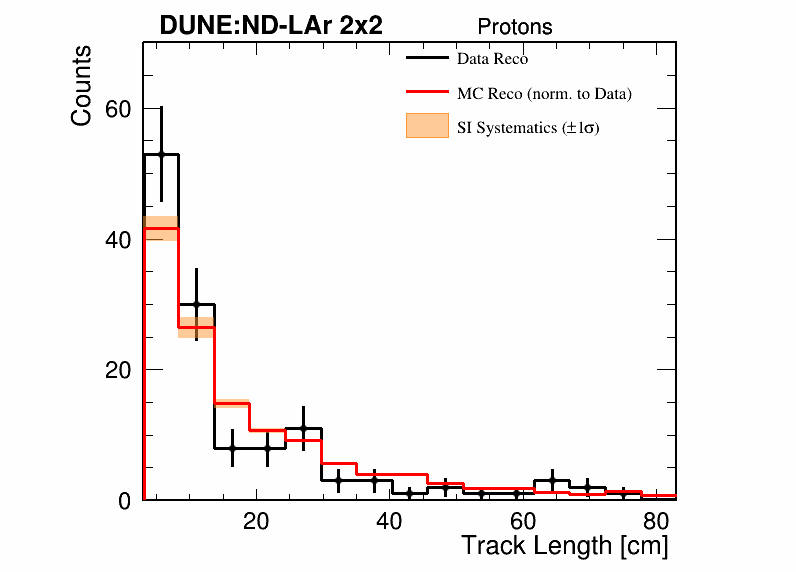
\includegraphics[width=0.50\textwidth]{fig16a_si}\hfill
    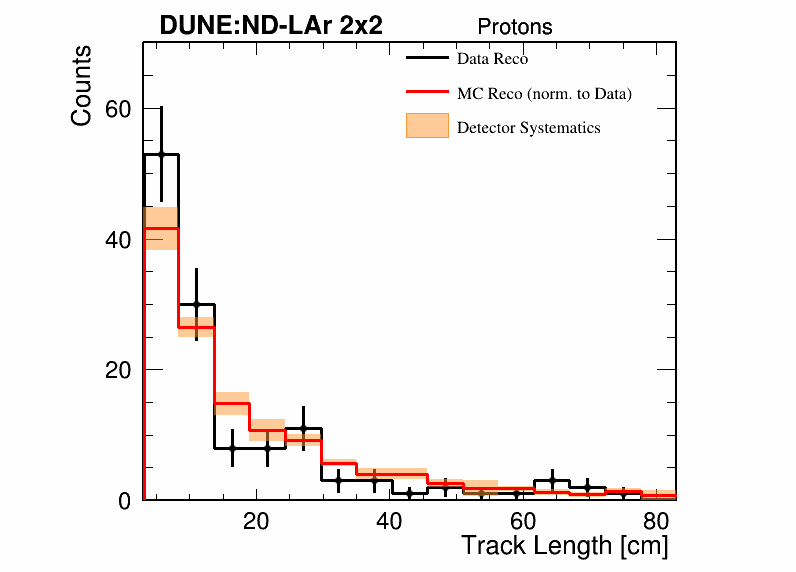
\includegraphics[width=0.50\textwidth]{fig16b_detector}\\[6pt]
    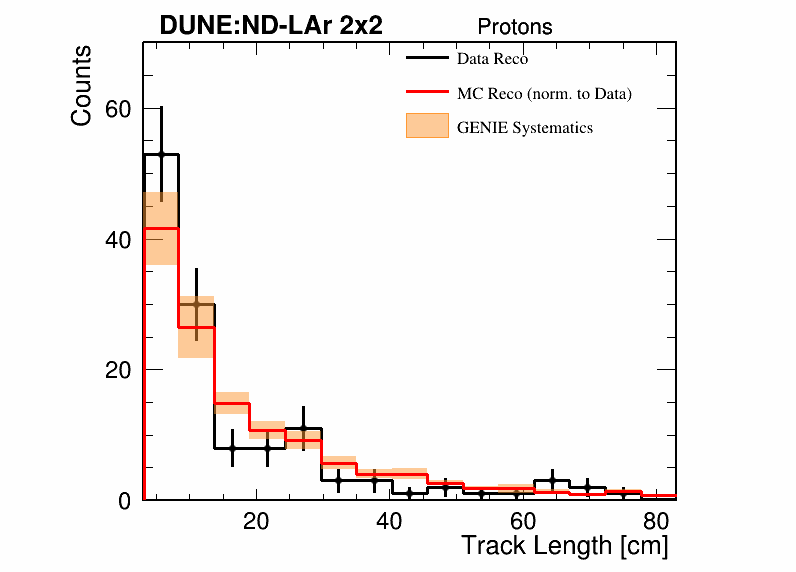
\includegraphics[width=0.50\textwidth]{fig16c_genie}\hfill
    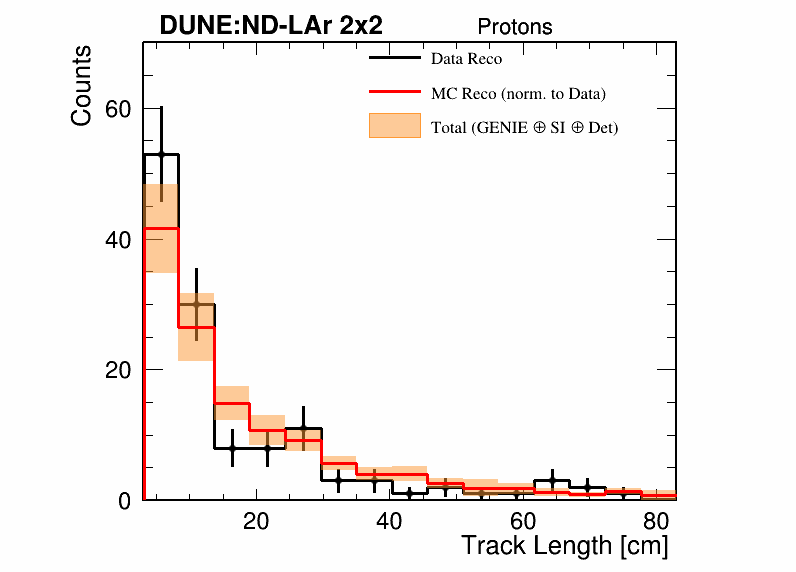
\includegraphics[width=0.50\textwidth]{fig16d_total}
    \caption{Reconstructed proton track length. Black: data. Red: simulation, normalized to data. Shaded bands:
    systematic uncertainty. Panels show the secondary-interaction band from G4RW
    at $\pm1\sigma$, the detector response band, the GENIE band, and their quadrature sum.}
    \label{fig:proton_si_band}
\end{figure}

Since the SI weight is defined at the level of the true \texttt{Geant4} trajectory, it can equally be applied to the true kinematics of the same backtracked candidates. Of the 3354 reconstructed proton candidates entering Fig.~\ref{fig:proton_si_band}, truth-backtracking identifies 2257 (67.3\%) as true protons, 622 (18.5\%) as $\pi^-$, 276 (8.2\%) as $\pi^+$, and 199 (5.9\%) as other species or without a truth match. Each candidate is weighted with the SI weights of its true species (proton, $\pi^+$ or $\pi^-$ weight file); the last group is not reweighted ($w=1$). Figure~\ref{fig:proton_truth_reco} shows the SI band for the 2257-candidate proton sample (top) and for the 1097 non-proton candidates (bottom) at both reconstructed and true track length, using raw MC counts with no normalization to data. Since these figures are not normalized to data, their bands should be compared with the band in Fig.~\ref{fig:proton_si_band} through their fractional width rather than their absolute size.


% SOURCE: slide 16, "Reconstructed vs. Truth Proton Track Length" (top row);
% non-proton panels (bottom row) from plot_truthProton_band.C
\begin{figure}[htb!]
    \centering
    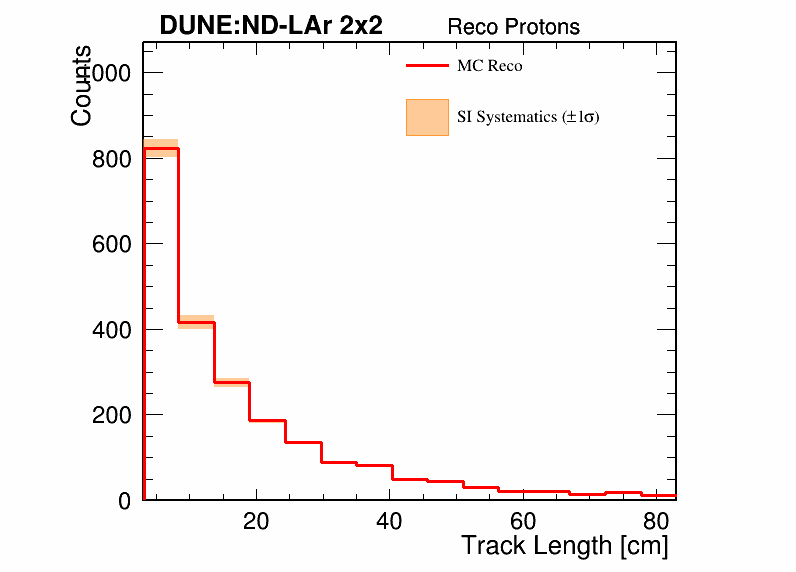
\includegraphics[width=0.50\textwidth]{fig18a_recoProton_raw_si}\hfill
    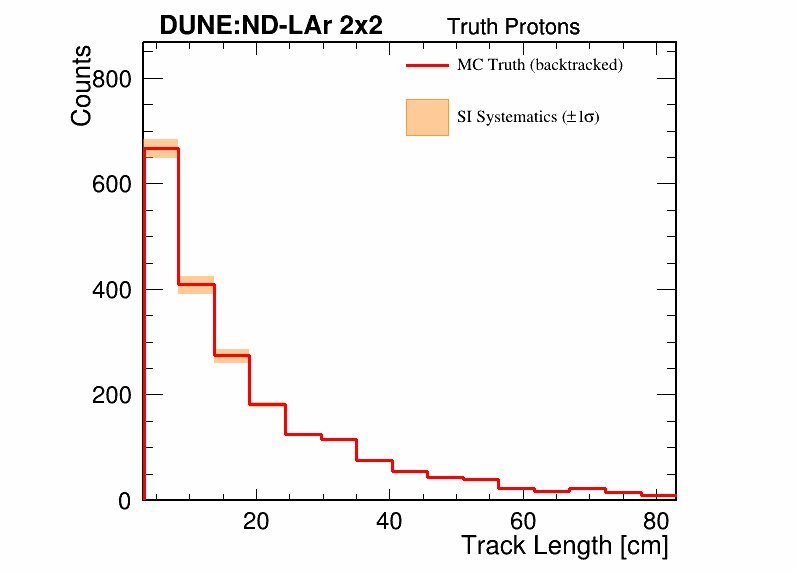
\includegraphics[width=0.50\textwidth]{fig18b_truthProton_raw_si}\\[4pt]
    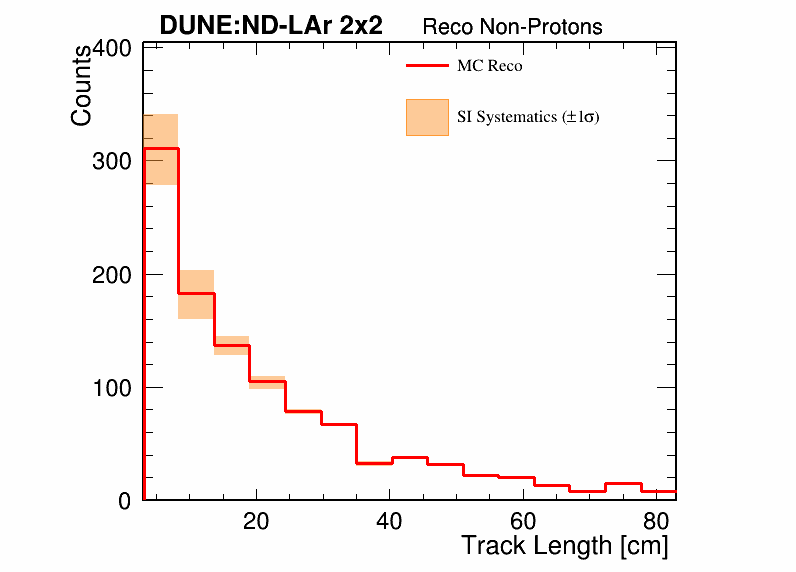
\includegraphics[width=0.50\textwidth]{fig18c_recoNonProton_raw_si}\hfill
    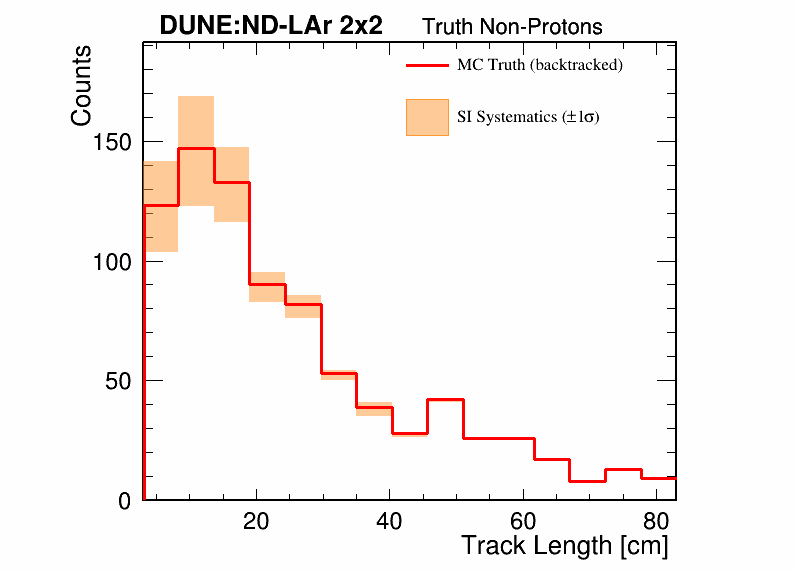
\includegraphics[width=0.50\textwidth]{fig18d_truthNonProton_raw_si}
    \caption{Reconstructed (left) and truth-level (right) track length, in raw MC counts not normalized to data, with the SI systematic band at $\pm1\sigma$. Top: the 2257 correctly-backtracked proton candidates. Bottom: the 1097 non-proton candidates at reconstructed level, and the 969 with a truth match (622 $\pi^-$, 276 $\pi^+$, 71 other species) at truth level; the remaining 128 have no truth match and appear only in the reconstructed-level panel.}
    \label{fig:proton_truth_reco}
\end{figure}

% The SI band is visibly the smallest of the three contributions across most of
% the distribution. That ordering is expected here: the proton selection is
% dominated by short tracks, and Figure~\ref{fig:proton_2d} shows the weight
% departs from unity only slowly with track length, so the shift is modest for the
% population that fills the leading bins.


\subsection{\label{subsec:next_physics}Example of Systematic Uncertainty Propagation in an older Multiplicity Analysis}

In this subsection, we incorporate the SI systematic uncertainties, along with nusystematics and detector response uncertainties, to an older version of multiplicity analysis \cite{azam_cm2025_multiplicity, docdb_37029} that is still useful to illustrate the individual systematic uncertainty contributions.

Figure~\ref{fig:multiplicity} shows all three systematic ingredients --- SI
from G4RW, GENIE interaction systematics~\cite{djurcic_nusyst_mr6p5}, and detector response
systematics~\cite{docdb_37843} --- applied to the charged-track multiplicity
distribution. The SI systematic band is negligible in the first bin
(multiplicity 1), since this bin is dominated by muons, which are insensitive
to secondary hadronic interactions.

% SOURCE: slide 19, "Next Step"
\begin{figure}[htb!]
    \centering
    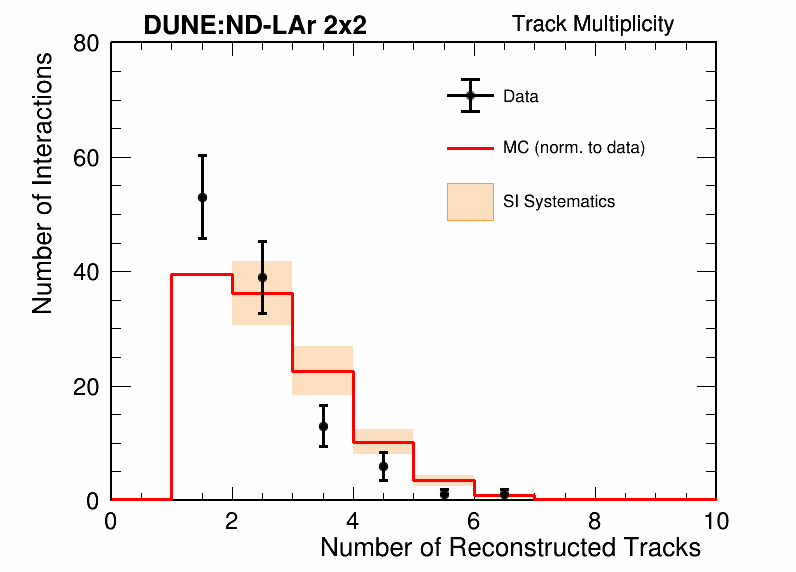
\includegraphics[width=0.50\textwidth]{fig17c_mult_si}\\[6pt]
    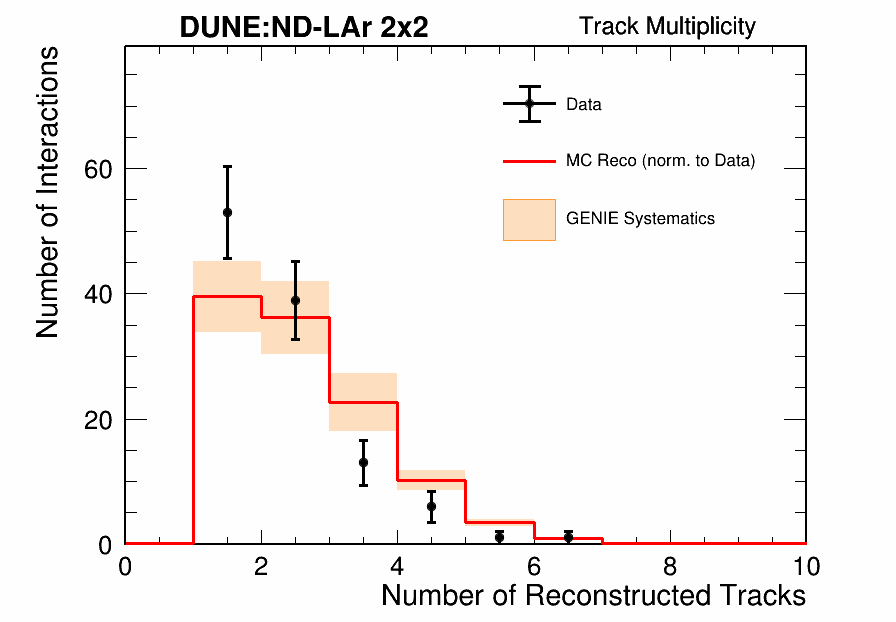
\includegraphics[width=0.50\textwidth]{fig17a_mult_genie}\hfill
    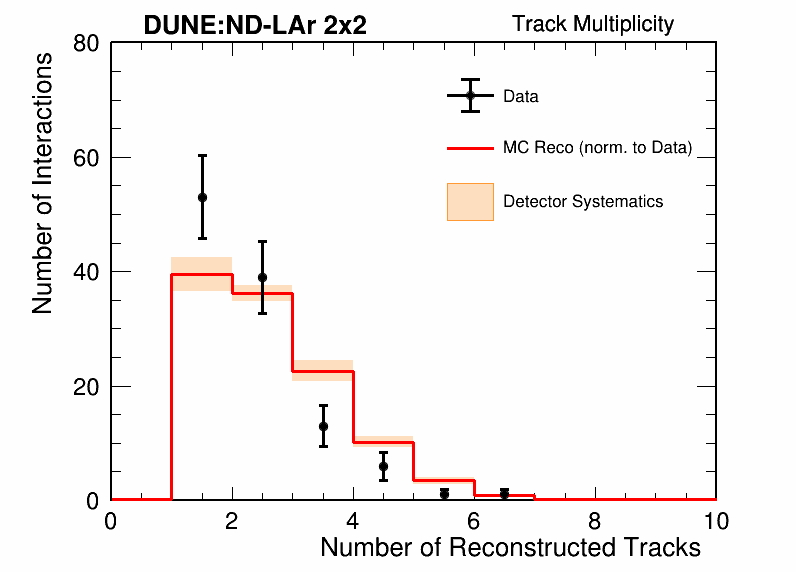
\includegraphics[width=0.50\textwidth]{fig17b_mult_detector}
    \caption{Reconstructed charged-track multiplicity with the
    secondary-interaction band from G4RW (top), the GENIE interaction
    systematic band (bottom left), and the detector response systematic band
    (bottom right). Black: data. Red: simulation, normalized to data.}
    \label{fig:multiplicity}
\end{figure}


% ===========================================================================
\section{\label{sec:locations}Software and File Locations}
% ===========================================================================

This section lists the software and file locations needed to reproduce the
work described in this note. All paths below are on NERSC. \texttt{\$CFS} abbreviates
\texttt{/global/cfs/cdirs/dune/users/mazam}.

% SOURCE: slide 17, "Current Status" (paths table)
\begin{table}[H]
\centering
\caption{Sample, weight, and input file locations.}
\label{tab:loc_samples}
\setlength{\tabcolsep}{12pt}
\begin{tabular}{ll}
\hline\hline
Item & Path \\
\hline
Patched EDepSim ($\pi^{\pm}$/$p$/$n$/$K^{\pm}$)
  & \texttt{\$CFS/EdepSim\_G4RW\_nu/patched\_withRock\_genieNu/} \\
G4RW weight outputs
  & \texttt{\$CFS/G4RW/output\_weights/patched\_withRock\_genieNu\_eq3p10/} \\
Fracs files ($\pi^{-}$, $p$, $n$)
  & \texttt{\$CFS/G4RW/G4Cascade/LAr\_*\_cascade\_*.root} \\
Fracs file ($\pi^{+}$, official)
  & \texttt{\$DUNE\_PARDATA\_DIR/Geant4ReweightInput/LAr\_PiPlus\_cascade\_0\_9000.root} \\
README files
  & \texttt{\$CFS/softwares/README} \\
\hline\hline
\end{tabular}
\end{table}


\begin{table}[H]
\centering
\caption{Software locations and the patched source files.}
\label{tab:loc_software}
\setlength{\tabcolsep}{18pt}
\begin{tabular}{ll}
\hline\hline
Item & Path \\
\hline
$2\times2$ G4RW pipeline      & \texttt{\$CFS/softwares/2x2\_g4rw/} \\
Custom \texttt{Geant4Reweight} build & \texttt{\$CFS/softwares/geant4reweight\_custom/} \\
Patch archive                 & \texttt{\$CFS/softwares/patches/} \\
EDepSim patch source          & \texttt{\$CFS/EdepSim\_G4RW/patch/EDepSimPersistencyManager.cc} \\
EDepSim production script     & \texttt{\$CFS/EdepSim\_G4RW/batch\_scripts/run\_g4rw\_edepsim\_batched.sh} \\
\hline\hline
\end{tabular}
\end{table}



% The patch archive is organised by the software each patch applies to:

% \begin{itemize}[nosep]
%   \item \texttt{patches/geant4reweight/} --- \texttt{G4ProtonReweighter.cc},
%         \texttt{G4NeutronReweighter.cc}, \texttt{G4ReweightParameterMaker.cc},
%         \texttt{G4Reweighter.cc} (the Eq.~\ref{eq:wi} correction).
%   \item \texttt{patches/fcl/geant4reweight/} --- cascade configurations for
%         proton, neutron, and $\pi^{-}$.
%   \item \texttt{patches/edepsim/} --- the patched
%         \texttt{EDepSimPersistencyManager.cc}.
%   \item \texttt{patches/2x2\_g4rw/} --- the weighting executable
%         (\texttt{do\_weighting\_v2.c++}), its FHiCL configurations,
%         \texttt{Makefile}, and batch scripts.
%   \item \texttt{patches/diagnostics/} --- the trajectory point-count macros
%         used for Table~\ref{tab:traj_points}.
% \end{itemize}

\begin{table}[H]
\centering
\caption{Software versions used. The two \texttt{boost} versions are
required at runtime: the locally built libraries link against
\texttt{v1\_80\_0} while the UPS dependency closure links against
\texttt{v1\_82\_0}, and both must be on \texttt{LD\_LIBRARY\_PATH}.}
\label{tab:loc_versions}
\setlength{\tabcolsep}{18pt}
\begin{tabular}{lll}
\hline\hline
Package & Version & Note \\
\hline
\texttt{2x2\_G4RW}      & commit \texttt{9bf2556} & \\
\texttt{edep-sim}       & tag \texttt{3.2.0.2x2.1} & patched, see Sec.~\ref{subsec:edepsim_patch} \\
\texttt{2x2\_sim}       & commit \texttt{7c62186} & geometry and run scripts \\
\texttt{Geant4Reweight} & \texttt{v01\_21\_02} & patched, see Sec.~\ref{subsec:code_changes} \\
\gfour{}                & \texttt{v4\_11\_2\_p02} & \\
ROOT                    & \texttt{v6\_28\_12} & \\
\texttt{cetmodules}     & \texttt{v3\_24\_01} & \\
\texttt{boost}          & \texttt{v1\_80\_0}, \texttt{v1\_82\_0} & both needed at runtime \\
\texttt{dune\_pardata}  & \texttt{v01\_84\_00} & official $\pi^{+}$ fracs file \\
\hline\hline
\end{tabular}
\end{table}

Two containers are used. The \texttt{Geant4Reweight} and $2\times2$ G4RW builds
run in \texttt{fermilab/fnal-wn-sl7:latest}, which supplies the Scientific Linux
7 environment and the DUNE UPS stack. The EDepSim build and production run in
\texttt{mjkramer/sim2x2:ndlar011}; this container is required rather than
optional, because the $2\times2$ GDML geometry contains \texttt{G4Torus} shapes
that fail with a mismatched \gfour{} version.

Currently, the entire codebase lives on NERSC and we plan to migration it to a GitHub repository, so that the
weight production chain is reproducible outside the NERSC environment. With these locations established, the
remainder of this section gives a short recipe for using the resulting
weights in a CAF analysis.


\subsection{\label{subsec:usage}Applying G4RW Weights in a CAF Analysis}

The following steps show how to look up the SI weight for a particle in a CAF analysis.

\begin{enumerate}
  \item[] \textbf{Step 1:} Use the G4RW weight files (one file per
    hadron species) from following path:
\begin{bashcode}
$CFS/G4RW/output\_weights/patched\_withRock\_genieNu\_eq3p10/
\end{bashcode}

  \item[] \textbf{Step 2:} Load the \texttt{g4rwEvt} tree of the required
    species into a lookup table keyed by
    (\texttt{file\_idx}, \texttt{event\_id}, \texttt{track\_id}), with the
    weight as the value.

  \item[] \textbf{Step 3:} For each track in the CAF analysis, build the key
    (\texttt{cafFileIdx}, \texttt{nu.id}, \texttt{prim.G4ID}) as defined in
    Table~\ref{tab:matching_key}, where \texttt{cafFileIdx} is the index of
    the CAF file in the processing order. In the multiplicity analysis code
    this is done as:
\begin{cppcode}
// interaction ID (nu.id)
g4rw_nu_id   = (long long)sr->mc.nu[biggestMatchIndex].id;
// index of the current file in the CAF chain
g4rw_fileIdx = caf_chain->GetTreeNumber();
// Geant4 track ID of the matched particle (prim.G4ID)
g4rw_G4ID    = sr->mc.nu[biggestMatchIndex].prim[partNumber].G4ID;
\end{cppcode}

  \item[] \textbf{Step 4:} Look up this key in the table from Step 2. If an
    entry is found, the corresponding weight is read from it; if not, the
    nominal weight $w=1.0$ is assigned to this track. Steps 2 and 4 are
    implemented as:
\begin{cppcode}
std::map<std::tuple<int,int,int>, std::array<double,2>> wmap;

TFile* f = TFile::Open(weightFile);
TTree* t = (TTree*)f->Get("g4rwEvt");
int file_idx, event_id, track_id;
double w_1p33, w_0p67;
t->SetBranchAddress("file_idx",    &file_idx);
t->SetBranchAddress("event_id",    &event_id);
t->SetBranchAddress("track_id",    &track_id);
t->SetBranchAddress("weight_1p33", &w_1p33);
t->SetBranchAddress("weight_0p67", &w_0p67);
for (long i = 0; i < t->GetEntries(); i++) {
    t->GetEntry(i);
    wmap[{file_idx, event_id, track_id}] = {w_1p33, w_0p67};
}

// per track: nominal weight unless an entry is found
std::array<double,2> w = {1.0, 1.0};
auto it = wmap.find({cafFileIdx, (int)nu_id, G4ID});
if (it != wmap.end()) w = it->second;
\end{cppcode}

  \item[] \textbf{Step 5:} Apply the weight to that track's kinematics
    (true or reconstructed). A worked implementation is available in the
    multiplicity analysis code~\cite{proton_plots_repo}.
\end{enumerate}


% ===========================================================================
\section{\label{sec:status}Summary}
% ===========================================================================

This note has documented the extension of G4RW to the $2\times2$ Demonstrator: patching
EDepSim to retain full trajectories of six hadron species $(\pi^\pm,p,n,K^\pm)$, extending the G4RW framework and its fracs
files to four hadronic species $(\pi^\pm,p,n)$, implementing the full interaction-step weight
formula. Currently, kaons have the EDepSim patch only; no reweighter class work, fracs file, or weight production is done for them; the patch is groundwork
so that the trajectories exist if kaon reweighting is taken up later. 
The SI systematics are then propagated to reconstructed proton (Fig.~\ref{fig:proton_si_band}) and multiplicity distributions (Fig.\ref{fig:multiplicity}) alongside GENIE and
detector systematics. We also parameterized the weight as a continuous
function of true track length for protons and $\pi^+$. Software and file locations for reproducing this
work are given in Section~\ref{sec:locations}.

With the secondary-interaction uncertainty now available for these
observables, the next phase of this work moves from developing the
systematic itself to using it in downstream physics analysis: unfolding
the reconstructed distributions, optimizing the hadron-multiplicity
selection, and other analysis steps that depend on having this systematic
in hand. This study will be revisited as improved cross-section measurements become available to inform the underlying uncertainties.

\iffalse
\subsection{\label{subsec:next_per_channel}Next Steps}

In this preliminary SI weight production, only the total inelastic cross section has been varied which moves all exclusive channels together by the
same factor (Section~\ref{subsec:fcl}). This is a single degree of freedom and
treats channels as perfectly correlated.
The next step is to vary channels independently, using the per-channel parameterisation.

The current unisim treatment of Section~\ref{subsec:application} produces a rank-one
covariance matrix. Every bin is perfectly correlated with every other, and the
band size depends on the scale factor chosen by hand. The standard alternative is multisim. Rather than a small set of fixed scale
factors, $N$ universes are generated with scale factors drawn from a Gaussian
centred on the \gfour{} nominal,
\begin{equation}
\label{eq:multisim_draw}
f_u \sim \mathcal{N}(1.0,\, \sigma_{\text{prior}}),
\qquad u = 1,\ldots,N,
\end{equation}
with a motivated $\sigma_{\text{prior}}$. The covariance is
then
\begin{equation}
\label{eq:multisim_cov}
C_{ij} = \frac{1}{N}\sum_{u=1}^{N}
         \left(h^{(u)}_i - h^{\text{nom}}_i\right)
         \left(h^{(u)}_j - h^{\text{nom}}_j\right),
\end{equation}
which has rank up to $\min(N, n_{\text{bins}})$ and therefore carries
bin-to-bin correlation structure that the unisim matrix cannot. The band is
normalized to the prior automatically, with no manual rescaling. Equation
\ref{eq:unisim_cov} is the $N = 1$ case of Eq.~\ref{eq:multisim_cov}.
\fi



\bibliographystyle{apsrev4-2}
\bibliography{references}

\end{document}
